\section{Ablation Study}
In our ablation study, we investigated the impact of various court-level training data configurations on the performance of our models in the binary classification judgment prediction task. We observed consistent trends across multiple experiments, particularly when analyzing the results from the full \texttt{\named} dataset in relation to subsets that excluded specific court cases. The performance metrics are detailed in Appendix Tables \ref{tab:binary-judgment-results-single-SCI-HCs-Tribunal}, \ref{tab:binary-judgment-results-multi-SCI-HCs-Tribunal}, \ref{tab:binary-judgment-results-single-SCI-HCs}, \ref{tab:binary-judgment-results-multi-SCI-HCs}, \ref{tab:binary-judgment-results-single-SCI}, \ref{tab:binary-judgment-results-multi-SCI}, \ref{tab:binary-judgment-results-ILDC-single}, and \ref{tab:binary-judgment-results-ILDC-multi}. 

Our findings indicate that models trained on High Court cases exhibited the best performance, likely due to the substantial representation of High Court data in the training set. However, when these models were evaluated on the ILDC dataset, a noticeable drop in performance was observed. This suggests that while the models excel in familiar contexts, they struggle to generalize to datasets with different characteristics or distributions.

We also conducted experiments on the ternary judgment prediction task, incorporating additional court cases, with results presented in Appendix Tables \ref{tab:judgment-prediction-ternary-sci-HCs}, \ref{tab:judgment-prediction-ternary-sci-hcs-tribunals}, and \ref{tab:judgment-prediction-ternary-sci-hcs-tribunals-dailyorders}. These experiments further reinforced the significance of including diverse court data and highlighted the benefits of utilizing large volumes of training data. 

Our findings emphasize the importance of a diverse and comprehensive dataset. Including a broad spectrum of court cases not only enhances the model's understanding of various judicial contexts but also significantly improves its performance metrics. In particular, the models trained on the most extensive datasets achieved an F1 score of around 90\%, underscoring the critical role of data diversity and volume in achieving high accuracy.

Overall, the ablation study illustrates that the diversity and volume of training data play a crucial role in enhancing model performance, particularly in the context of legal judgment prediction tasks. Future work should continue to explore the impact of various data configurations to further optimize model accuracy and generalization capabilities.

%%%%%%%%%%%%%%%%%%%%%%%%%%%%%%%%%%%
\section{Rating Score Description}
\label{section:rating-score-description}
The evaluation of the explanations generated by the models was conducted using a 1–5 Likert scale, where each score reflects the quality and relevance of the provided explanation. The criteria for rating are as follows:

\textbf{[1]:} The explanation is entirely incorrect or fails to provide any relevant information. This score indicates that the response does not address the case judgment in any meaningful way.

\textbf{[2]:} The response is irrelevant or demonstrates a misunderstanding of the case judgment. A rating of 2 suggests that while some effort was made to respond, the explanation does not accurately reflect the case details.

\textbf{[3]:} The explanation is partially accurate but lacks critical details. This score indicates that the response contains some correct information, but it is insufficient for a complete understanding of the case judgment.

\textbf{[4]:} The response is generally accurate and relevant, comparable to the ground truth. A rating of 4 signifies that the explanation aligns well with the expected outcomes and provides a solid understanding of the case.

\textbf{[5]:} The explanation is fully accurate, relevant, and potentially superior to the expert's explanation. This highest rating reflects an exceptional response that not only meets the criteria of accuracy and relevance but also offers insights that exceed standard expert evaluations.

\section{Experimental Setup and Hyper-parameters}
\label{sec:Experimental-setup}

\subsection{Transformers Training Hyper-parameters}
For model training, we used a batch size of 16, the Adam optimizer \cite{kingma2014adam}, and a learning rate of 2e-6. The training was conducted over 3 epochs on the \texttt{\named} train dataset. The remaining hyperparameters were set to their default values as provided by the HuggingFace library.

\subsection{\namel Training Procedure}
The fine-tuning of the \texttt{\namel} model was conducted using the LLaMa 2 7B model architecture, with the model loaded in Bfloat16 precision. The training was done in Google Colab Pro, utilizing a single A100 GPU with 40GB of memory. Given the constraints of limited computational resources, we carefully selected parameters to fully utilize the available compute power. This setup enabled us to develop a highly capable model within a reasonable time frame of 48 hours, incurring a cost of approximately \$59. During the training process, the maximum token length was set at 2,096. We employed the Low-Rank Adaptation (LoRA) technique, initializing the LoRA rank at 16 and setting the alpha parameter to 64, with a dropout rate of 0.1. This configuration was applied to all layers of the model, aiming to achieve performance comparable to a fully fine-tuned model. The integration of flash-attention 2 significantly improved the training speed.

The optimization process utilized a Paged Adam 32-bit optimizer with a learning rate of 1e-4, alongside a ``cosine" learning rate scheduler. The gradient accumulation steps were set to 4, and the warm-up ratio was established at 0.05. We employed DeepSpeed Stage 3 optimization, with a per-device batch size of 4. The model was trained for a total of 3,000 steps, which corresponds to approximately 0.347 epochs.

% The entire training process was meticulously tracked using Weights \& Biases \cite{wandb}, allowing for detailed monitoring and analysis. The progression of training and evaluation losses during the fine-tuning process is illustrated in Appendix Figures \ref{fig:llama2_cpt_train}, \ref{fig:llama2_cpt_val}, \ref {fig:sft_pred_train}, \ref{fig:sft_pred_val}, \ref{fig:sft_pred_expl_train} and \ref{fig:sft_pred_expl_val}. These figures highlight the model's loss trends during the Continued Pretraining (CPT) and Supervised Fine-Tuning (SFT) phases, for both prediction-only and prediction-with-explanation tasks. Notably, the CPT phase shows a consistent reduction in training and evaluation losses, indicating the model's ability to learn effectively from the legal corpus. Similarly, the SFT phase results display refined loss curves, especially in the prediction-with-explanation task, suggesting the model's enhanced capability to generate comprehensive and accurate legal explanations.

\section{Hallucination}
\label{sec:hallucination}
In our study, we address the issue of hallucinations in model-generated text, which is a prevalent challenge when using large language models for generating legal judgments. Hallucinations occur when the model produces information that is false or irrelevant, not supported by the input data. A sample of hallucination has been provided in Appendix Table \ref{cpt-hallucination-example}. To tackle this issue, we employed a specialized fine-tuning strategy aimed at significantly reducing such errors. A detailed comparative analysis provided in Appendix \ref{subsec:CPT-hallucination} 
 - CPT LLaMa-2 hallucinations, which 
 highlights the effectiveness of these strategies. This analysis illustrates how fine-tuning and instruction-tuning, specifically tailored to the legal domain, can help minimize hallucinations, resulting in outputs that are clearer, more accurate, and legally coherent.

% \subsection{Hallucination Example}
% \label{sec:Hallucination-example}

\subsection{CPT LLaMa-2 hallucinations}
\label{subsec:CPT-hallucination}
In the subsection, we conduct a thorough comparison between ground truth and fine-tuned models to demonstrate some samples where the CPT model showed signs of hallucination. Table \ref{cpt-hallucination-example} in the Appendix presents an extensive analysis of the model, illustrating the performance of the LLaMa-2 pre-trained model on legal judgment prediction with explanation tasks in our PredEx dataset. In the given table, this can be observed that the model did not only produce incorrect judgment but also delivered the wrong explanation, if not repeating the sentences and printing a random repetitive set of numbers. Some examples in the table show the model hallucinating by repeating a statement irrelevant to the case information. This comparison specifically focuses on how instruction-tuning can mitigate the issues of inaccuracies often found in the responses generated by pre-trained Large Language Models (LLMs).

\subsection{CPT LLaMa-2 vs \namel (CPT+SFT)}
\label{subsec:CPT-vs-SFT}
In the subsection, we conduct a detailed comparison between LLaMa-2-7B CPT and \namel (CPT+SFT) to demonstrate some samples where the fine-tuned model \namel performed better than LLaMa-2 CPT in all aspects including prediction and explanation. Table \ref{tab:ca_analysis} in the Appendix presents an extensive analysis of the model, illustrating the performance of the LLaMa-2 pre-trained model against the \namel model on legal judgment prediction with explanation tasks in our PredEx dataset. In the given table, it can be observed that the performance of the LLaMa-2 CPT looks good at once but when we refer to the explanation, we realize that the explanation given for the prediction does not follow the context of the legal judgment. On the other hand, \namel maintains the contextual information and retains a lot of information from the legal judgment.As a result, \namel outperforms the LLaMa-2 CPT with better context information and reasonable facts inclusion.

%%%%%%%%%%%%%%%%%%%%%%%%%%%%%%%%%%
% hallucination_table
%%%%%%%%%%%%%%%%%%%%%%%%%%%%%%%%%%

\begin{table*}[ht]
\centering
\tiny
\resizebox{\textwidth}{!}{%
\begin{tabular}{|c|l|}
\hline

\textbf{Model} &
  \multicolumn{1}{c|}{\textbf{Decision and Explanation}} \\ \hline
 
Ground Truth &
  { \begin{tabular}[c]{@{}l@{}}Decision: Rejected. \\Explanation:
  \\IT first requires to be noticed that the above two agreements\\ dated November 1, 1966 and may 13, 1967, are agreements made otherwise \\than in the course of conciliation proceedings and are of the nature referred\\ to in(1) of S. 18 Admittedly, these agreements were not signed on behalf of\\ the workmen who were were not members of the 2nd respondent Union.\\  .........................\\ As we are unable to accept that contention, the third contention alsowe\\ have held that these agreements have ceased to be in operation and did \\not require to be terminated, this contention must fail. We have\\ already recorded reasons in that connection in the previous discussion.\end{tabular}} \\ \hline
Llama2-7B CPT &
  { \begin{tabular}[c]{@{}l@{}}Decision: No clear decision generated.\\ Explanation:\\ 1.0 The order is upheld. 1.1 The order is upheld. 1.2 The order is upheld. \\1.3 The order is upheld. 1.4 The order is upheld. 1.5 The order is upheld.\\ 1.6 The order is upheld. 1.7 The order is upheld. 1.8 The order is upheld. \\1.9 The order is upheld. 1.10 The order is upheld. ............. \\1.73 The order is upheld. 1.74 The order is upheld. 1.75 The order is upheld. \\1.76 The order is upheld. 1.77 The order is upheld. 1.78 The order is upheld.\\ 1.79 The order is upheld. 1.80 The order is upheld. 1.81 The order is upheld.\\ 1.82 The order is upheld. 1.83 The order is upheld. 1.\end{tabular}} \\ \hline

Ground Truth &
  { \begin{tabular}[c]{@{}l@{}}Decision: Rejected \\ Explanation: 
  \\For proper appreciation of the contentions advanced by the parties\\ before us, it is necessary to refer to some of the provisions of the Act.\\ Section 160(1)(i) of the Act prov ides that in respect of the income of\\ a non-resident specified in sub-section (1) of section 9 of the Act, the\\ agent of the non-resident, including a person who is treated as\\ an agent under section 163 is a representative assessee\\...................\\The above cable shows that the London Solicitors had sought information about\\ the suits in Calcutta t o enable them to engage Mr. Blanco White to plead\\ on behalf of the German Corporation in the said suits. On December 23, 1969,\\ the London Solicitors wrote a letter to the appellants in which it\\ was stated that the copies of certain documents sent by the appellants had\\ been handed over to Mr. Blanco White in addition to copies of certain\\ other documents which they themselves had handed over to him.\end{tabular}} \\ \hline
Llama2-7B CPT &
  {\begin{tabular}[c]{@{}l@{}}Decision: Rejected \\Explanation:
  \\The appellants are a partnership firm and the partners are Mr. and\\ Mr. D.K.Jain. Mr. D.K.Jain is a non-resident Indian.Income from the\\ partnership firm is subject to tax in India under the provisions of the\\ Income-tax Act, 1961....................The firm has no in Germany.The firm has no\\ in Germany.The firm has no in Germany.The firm has\\ no in Germany.The firm has no in Germany.The firm has no in Germany.The\\ firm has no in Germany.The firm has no in Germany.The firm has no in\\ Germany.The firm has no in Germany.The firm has no in Germany.The\end{tabular}} \\ \hline
\end{tabular}%
}
\caption{We observe 'reject' judgments in the response generated by LLaMa-7B CPT with varying explanations, conclusions, and repeating responses.}
\label{cpt-hallucination-example}
\end{table*}
%%%%%%%%%%%%%%%%%%%%%%%%%%%%%%%%%%%%%%%%%%%%%%%%%%


%%%%%%%%%%%%%%%%%%%%%%%%%%%%
\begin{table*}[t]
\centering
\resizebox{\textwidth}{!}{%
\begin{tabular}{|c|l|l|ll}
\cline{1-3}
\textbf{Model}                                                                          & \multicolumn{1}{c|}{\textbf{Decision and Explanation}}                  & \multicolumn{1}{c|}{\textbf{Explanation of error}}                      &  &  \\ \cline{1-3}
Ground Truth                                                                                & {\begin{tabular}[c]{@{}l@{}}Case decision: Accepted\\ Explanation: \\ In our opinion, the High Court should have examined these\\ questions and especially the question as to whether the had been able to\\ substantiate the claim that it was in possession of the entire underground \\rights in respect of Ac.covered by the agreement of 1934. The agreement\\ of 1934 bound the Government and the Hindu undivided family: the was \\not a party to it. Even if the Hindu undivided family continued in\\ possession of some of the mines, seams and veins after October 1, 1947,\\ it is a moot question whether such possession meant possession of the\\ seams, mines, and veins which were not actually being worked. A further\\ question would arise as to how and what right the company could lawfully\\ claim in respect of the colliery by virtue of the deed of assignment in 1950.\\ Without an adjudication of these questions the High Court was not justified\\ in directing the State and other authorities to put the company in possession\\ of the area described as a virgin area. Whether the case is a fit for\\ examination on affidavits will be for the High Court to consider.\end{tabular}} & &  &  \\ \cline{1-3}
Llama-2-7B CPT                                                                                  & { \begin{tabular}[c]{@{}l@{}}Case decision: Accepted\\ Explanation: 
\\1.The petitioner was in actual physical of the area which was\\ taken over by the State Government on February 28, 1970. The High\\ Court was not justified in directing the State and other authorities to\\ put the petitioner in the physical area. The State Government had\\ taken over the area for the purpose of the public interest. The High Court\\ should have refrained from granting any relief to the petitioner.
\\2. The respondent company was not in actual physical of the area which\\ was taken over by the State Government on February 28, 1970. The High\\ Court was not justified in directing the State and other authorities to put\\ the petitioner in physical of the area. The State Government had taken\\ over the area for the purpose of the public interest. The High Court\\ should have refrained from granting any relief to the petitioner.
\\
...
\\12. The High Court should have examined the questions of whether the\\ petitioner was in actual physical of the area which was taken over by\\ the State Government on February 28, 1970, and whether the State\\ Government had taken over the area for the purpose of the public\\ interest. The High Court should have refrained from granting any\\ relief to the petitioner.
\\13 The High Court should have examined the questions whether the\\ petitioner was in actual physical of the area which was taken\end{tabular}}                                                     

& \begin{tabular}[c]{@{}l@{}} The vanilla incorrectly explains the\\ explanation of the case text. The reason\\ behind hallucination is lack of contextual\\ understanding of the case information,\\ overemphasis on certain parts of the\\ input, and missing information such as\\ the agreement of 1934 and 1950. One of the\\ reasons could also be the complex legal\\ language that the model could not fully grasp.
\end{tabular} &  &  \\ \cline{1-3}

\begin{tabular}[c]{@{}c@{}}\namel \\ (CPT+SFT)\\ Instruction-tuning\\ for prediction \\ with explanation\\ task\end{tabular} & \begin{tabular}[c]{@{}l@{}}Case decision: Accepted\\ Explanation: \\ Further there was no agreement as regards the royalties\\ to be paid under the renewed lease.
\\23. With regard to the right claimed under the deed of assignment\\ it was argued that the assignment could take place only when the\\ lease was in force and as the lease of 1917 had expired in 1947\\ no valid assignment could be taken place if indeed, there was, in fact, \\ any assignment of the colliery as alleged.
\\24. It was urged that without examining those questions and without\\ coming to the conclusion that the petitioner-company had by their\\ petition disclosed a legal right in them with regard to the colliery\\ or to continue in possession thereof the High Court was not competent\\ to grant them any relief as it had purported to do. It was submitted\\ that at the most there was a term in the agreement of 1934 read with\\ the lease of 1917 which entitled the Hindu undivided family to sue\\ for specific performance of the contract to renew for a further term.\\ The demise in its favor of the veins etc., under the lease of 1917 had\\ come to an end and even if the person in possession of the seams\\ and veins which were being worked could not be dispossessed by an\\ order of the nature disclosed in the letter of February 1970, the \\petitioner-company had not been able to show any right in it to claim\\ possession of the virgin area, that it to say, the seems, veins, mines\\, etc., of which they were not in physical possession and which they\\ were not working at the moment, when the impugned order was served on\\ them.
\\25. In our opinion, the High Court should have examined these questions\\ and especially the question as to whether the petitioner-company had been\\ able to substantiate the claim that it was in possession of the entire\\ underground rights in respect of Ac. 871-49 covered by the agreement\\ of 1934. The agreement of 1934 bound the Government and the Hindu\\ undivided family: the petitioner company was not a party to it. Even if\\ the Hindu undivided family continued in possession of some of the mines\end{tabular}                                      & \begin{tabular}[c]{@{}l@{}}The Finetuned model correctly explains\\ the reasoning behind the case judgment \\ comparatively better. The reasoning contains\\ better context information and is organized\\ logically. This explanation includes specific legal\\ arguments related to the agreements.\\ The explanation also compares the petitioner's\\ claim with actual agreements and classes. \end{tabular}&  &  \\ \cline{1-3}
\end{tabular}%
}
\caption{Comparative analysis of responses generated by LLaMa-2-7B (CPT) and \namel (CPT+SFT).}
\label{tab:ca_analysis}
\end{table*}
%%%%%%%%%%%%%%%%%%%%%%%%%
% %%%%%%%%%%%%%%%%%%%%%%%%%%%%%%%%%%%%
%%%%%%%%%%%%%%%%%%%%%%%%%
% Indian Case Structure Example
%%%%%%%%%%%%%%%%%%%%%%%%%

% \section{Indian Case Structure Example}

\begin{table*}[t]
\centering
\resizebox{\textwidth}{!}{%
\begin{tabular}{|
>{}l |}
\hline
\textbf{CASE NO:} \\ \hline
 CIVIL APPEAL NOS. 3088-3089 OF 2020\\ \hline
\textbf{APPELLANTS:} \\ \hline
BHARTI AIRTEL LIMITED AND ANOTHER  \\ \hline
\textbf{RESPONDENT:} \\ \hline
VIJAYKUMAR V. IYER AND OTHERS \\ \hline
\textbf{DATE OF JUDGMENT:} \\ \hline
03/01/2024 \\ \hline
{ \textbf{BENCH:}} \\ \hline
{ Dipankar Datta} \\ \hline
\textbf{CASE TEXT:} \\ \hline

{ \begin{tabular}[c]{@{}l@{}}
... The present appeals raise an interesting question on the right to claim set-off in the Corporate Insolvency \\Resolution Process when the Resolution Professional proceeds in terms of clause (a) to sub-section (2) of\\ \textcolor{blue}{Section 25 of the Insolvency and Bankruptcy Code, 20161} to take custody and control of all the assets of \\the corporate debtor .... \\ \\ 

...The NCLAT vide order dated 17th May 2019 allowed the appeal, inter alia, holding that set-off is violative of the \\basic principles and protection accorded under any insolvency law. Set-off is antithetical to the objective of the IBC. \\Reference was made to the non-obstante provisions in the form of \textcolor{blue}{Section 238 of the IBC}. As moratorium under\\ \textcolor{blue}{Section 14(4)} applies till the date of completion of the Corporate Insolvency Resolution Process, which is till the\\ resolution plan...  \\ \\ 

...The judgment of this Court in The \textcolor{magenta}{Official Liquidator of High Court of Karnataka v. Smt. V. Lakshmikutty53} \\ had applied \textcolor{blue}{Section 46 of the Provincial Insolvency Act, 1920} and had accordingly permitted insolvency \\set-off on interpretation and application of \textcolor{blue}{Sections 529 and 530 of the Companies Act, 1956}. In that context, \\it is observed that the English courts, on \textcolor{magenta}{52 Career Institute Educational Society v. Om Shree Thakurji Educational}\\ \textcolor{magenta}{Society, 2023} SCC OnLine SC 586....\\ \\ 


... Thereupon the Airtel entities made a payment of Rs.341.80 crores due to the Aircel entities on 10th January 2019.\\ The balance amount of Rs.145.20 crores was set-off by the Airtel entities on the ground that this amount was owned\\ by the Aircel entities to the Airtel entities. According to Airtel entities, Rs.145.20 crores was the adjusted or the net \\amount payable by the Aircel entities towards operational charges, SMS charges and interconnect usage charges to\\ the Airtel entities ...\end{tabular}} \\ \hline
\textbf{JUDGEMENT:} \\ \hline
{ \begin{tabular}[c]{@{}l@{}}.... Having considered the contentions raised by the appellant Airtel entities in detail, and in light of the provisions\\ of the IBC relating to the Corporate Insolvency Resolution Process, \textcolor{red}{we do not find any merit in the present appeals}\\ \textcolor{red}{and the same are dismissed}. There will be no order as to costs....\end{tabular}} \\ \hline
\end{tabular}%
}
\caption{Example of Indian Case Structure. Sections referenced are highlighted in blue, previous judgments cited are in magenta, and the final decision is indicated in red.}
\label{case-example}
\end{table*}
%%%%%%%%%%%%%%%%%%%%%%%%%%%%%%%%%%%%%%%%%%%%%%%


%%%%%%%%%%%%%%%%%%%%%%%%%%%%%%%%%%%%%%%%%%%%%%%
\begin{table*}[ht]
%\small
    \centering
    \begin{tabular}{|p{0.8\textwidth}|}
    \hline
{\bf Template 1 (prediction + explanation)}\\
\hline
   
{\bf prompt} = f``````Task: Given a Supreme Court of India case proceeding enclosed in angle brackets $<$ $>$, your task is to predict the decision of the case (with respect to the appelant) and provide an explaination for the decision.\\


{\bf Prediction}: Given a case proceeding, the task is to predict the decision 0 or 1, where the label 1 corresponds to the acceptance of the appeal/petition of the appellant/petitioner and the label 0 corresponds to the rejection of the appeal/petition of the appellant/petitioner,  Explanation: The task is to explain how you arrived at the decision by predicting important sentences that lead to the decision. \\


{\bf Context}: Answer in a consistent style as shown in the following two examples: \\


  {\bf case\_proceeding}: \# case\_proceeding example 1\\


  {\bf Prediction}: \# example 1 prediction \\


  {\bf Explanation}: \# example 1 explanation\\


  {\bf case\_proceeding}: \# case\_proceeding example 2\\


 {\bf  Prediction}: \# example 2 prediction\\


 {\bf Explanation}: \# example 2 explanation\\


{\bf Instructions}: Learn from the above two examples and perform the task for the following case proceeding. \\


case\_proceeding: $<$\{case\_proceeding\}$>$\\


Format your output in list format: [prediction, explanation]''''''\\

\hline
    {\bf Template 2 (prediction only)}\\
    \hline
   
{\bf prompt} = f``````Task: Given a Supreme Court of India case proceeding enclosed in angle brackets $<$ $>$, your task is to predict the decision of the case (with respect to the appellant).\\


{\bf Prediction}: Given a case proceeding, the task is to predict the decision 0 or 1, where the label 1 corresponds to the acceptance of the appeal/petition of the appellant/petitioner and the label 0 corresponds to the rejection of the appeal/petition of the appellant/petitioner \\


{\bf Context}: Answer in a consistent style as shown in the following two examples: \\


  {\bf case\_proceeding}: \# case\_proceeding example 1\\


  {\bf Prediction}: \# example 1 prediction \\


 


  {\bf case\_proceeding}: \# case\_proceeding example 2\\


  {\bf Prediction}: \# example 2 prediction\\


 


{\bf Instructions}: Learn from the above two examples and perform the task for the following case proceeding. \\


{\bf case\_proceeding}: $<$\{case\_proceeding\}$>$\\


Give the output predicted case decision as either 0 or 1.''''''\\

\hline

    \end{tabular}
    \caption{Prompts for Judgment Prediction taken from \cite{vats-etal-2023-llms}.}
    \label{tab:judgment_prediction_prompts_few}
\end{table*}
%%%%%%%%%%%%%%%%%%%%%%%%%%%%%%%%%%%%%%%%%%%%%%%

%%%%%%%%%%%%%%%%%%%%%%%%%%%%%%%%%%%%%%%%%%%%%%%
\begin{table*}[ht]
%\small
    \centering
    \begin{tabular}{|p{0.8\textwidth}|}
    \hline
    {\bf Template 3 (prediction only)}\\
    \hline
   
{\bf prompt} = f``````
\#\#\# {\bf Instructions}: Analyze the case proceeding and predict whether the appeal/petition will be rejected (0) or accepted (1). \\

\#\#\# \textbf{Input}: $<$\{case\_proceeding\}$>$\\


\#\#\# Response:
  ''''''\\
\hline
    {\bf Template 4 (prediction with explanation)}\\
    \hline
   
{\bf prompt} = f``````
\#\#\# {\bf Instructions}: Analyze the case proceeding and predict whether the appeal/petition will be accepted (1) or rejected (0), and subsequently provide an explanation behind this prediction with important textual evidence from the case. \\

\#\#\# \textbf{Input}: $<$\{case\_proceeding\}$>$\\


\#\#\# Response:
  ''''''\\
\hline


    \end{tabular}
    \caption{Prompts for Judgment Prediction used for instruction fine-tuned models taken from \cite{nigam2024legaljudgmentreimaginedpredex}. Instructions were randomly chosen from Table \ref{Instruction-sets}.}
    \label{tab:judgment_prediction_prompts_zero}
\end{table*}
%%%%%%%%%%%%%%%%%%%%%%%%%%%%%%%%%%%%%%%%%%%%%%%

%%%%%%%%%%%%%%%%%%%%%%%%%%%%%%%
\begin{table*}[ht]
\centering
\resizebox{0.95\textwidth}{!}{%
\tiny
\begin{tabular}{|cl|}
\hline
\multicolumn{2}{|c|}{\textbf{\textcolor{blue}{Instruction sets for Predicting the Decision}}} \\ \hline
\multicolumn{1}{|c|}{1} &
  Analyze the case proceeding and predict whether the appeal/petition will be accepted (1) or rejected (0). \\ \hline
\multicolumn{1}{|c|}{2} &
  \begin{tabular}[c]{@{}l@{}}Based on the information in the case proceeding, determine the likely outcome: acceptance (1) or \\ rejection (0) of the appellant/petitioner's case.\end{tabular} \\ \hline
\multicolumn{1}{|c|}{3} &
  Review the case details and predict the decision: will the court accept (1) or deny (0) the appeal/petition? \\ \hline
\multicolumn{1}{|c|}{4} &
  \begin{tabular}[c]{@{}l@{}}Considering the arguments and evidence in the case proceeding, predict the verdict: is it more likely to be in \\ favor (1) or against (0) the appellant?\end{tabular} \\ \hline
\multicolumn{1}{|c|}{5} &
  \begin{tabular}[c]{@{}l@{}}Examine the details of the case proceeding and forecast if the appeal/petition stands a chance of being \\ upheld (1) or dismissed (0).\end{tabular} \\ \hline
\multicolumn{1}{|c|}{6} &
  \begin{tabular}[c]{@{}l@{}}Assess the case proceedings and provide a prediction: is the court likely to rule in favor of (1) or against (0)\\ the appellant/petitioner?\end{tabular} \\ \hline
\multicolumn{1}{|c|}{7} &
  \begin{tabular}[c]{@{}l@{}}Interpret the case information and speculate on the court's decision: acceptance (1) or rejection (0) of the \\ presented appeal.\end{tabular} \\ \hline
\multicolumn{1}{|c|}{8} &
  \begin{tabular}[c]{@{}l@{}}Given the specifics of the case proceeding, anticipate the court's ruling: will it favor (1) or oppose (0) the \\ appellant’s request?\end{tabular} \\ \hline
\multicolumn{1}{|c|}{9} &
  \begin{tabular}[c]{@{}l@{}}Scrutinize the evidence and arguments in the case proceeding to predict the court's decision: will the appeal\\  be granted (1) or denied (0)?\end{tabular} \\ \hline
\multicolumn{1}{|c|}{10} &
  \begin{tabular}[c]{@{}l@{}}Analyze the legal arguments presented and estimate the likelihood of the court accepting (1) or rejecting (0) \\ the petition.\end{tabular} \\ \hline
\multicolumn{1}{|c|}{11} &
  \begin{tabular}[c]{@{}l@{}}From the information provided in the case proceeding, infer whether the court's decision will be positive (1) \\ or negative (0) for the appellant.\end{tabular} \\ \hline
\multicolumn{1}{|c|}{12} &
  \begin{tabular}[c]{@{}l@{}}Evaluate the arguments and evidence in the case and predict the verdict: is an acceptance (1) or rejection\\ (0) of the appeal more probable?\end{tabular} \\ \hline
\multicolumn{1}{|c|}{13} &
  \begin{tabular}[c]{@{}l@{}}Delve into the case proceeding and predict the outcome: is the judgment expected to be in support (1) or \\ in denial (0) of the appeal?\end{tabular} \\ \hline
\multicolumn{1}{|c|}{14} &
  \begin{tabular}[c]{@{}l@{}}Using the case data, forecast whether the court is likely to side with (1) or against (0) the \\ appellant/petitioner.\end{tabular} \\ \hline
\multicolumn{1}{|c|}{15} &
  \begin{tabular}[c]{@{}l@{}}Examine the case narrative and anticipate the court's decision: will it result in an approval (1) or \\ disapproval (0) of the appeal?\end{tabular} \\ \hline
\multicolumn{1}{|c|}{16} &
  \begin{tabular}[c]{@{}l@{}}Based on the legal narrative and evidentiary details in the case proceeding, predict the court's stance: \\ favorable (1) or unfavorable (0) to the appellant.\end{tabular} \\ \hline
\multicolumn{2}{|c|}{\textbf{\textcolor{blue}{Instruction sets for Integrated Approach for Prediction and Explanation}}} \\ \hline
\multicolumn{1}{|c|}{1} &
  \begin{tabular}[c]{@{}l@{}}First, predict whether the appeal in case proceeding will be accepted (1) or not (0), and then explain the \\ decision by identifying crucial sentences from the document.\end{tabular} \\ \hline
\multicolumn{1}{|c|}{2} &
  \begin{tabular}[c]{@{}l@{}}Determine the likely decision of the case (acceptance (1) or rejection (0)) and follow up with an \\ explanation highlighting key sentences that support this prediction.\end{tabular} \\ \hline
\multicolumn{1}{|c|}{3} &
  \begin{tabular}[c]{@{}l@{}}Predict the outcome of the case proceeding (1 for acceptance, 0 for rejection) and subsequently provide an\\  explanation based on significant sentences in the proceeding.\end{tabular} \\ \hline
\multicolumn{1}{|c|}{4} &
  \begin{tabular}[c]{@{}l@{}}Evaluate the case proceeding to forecast the court's decision (1 for yes, 0 for no), and elucidate the \\ reasoning behind this prediction with important textual evidence from the case.\end{tabular} \\ \hline
\multicolumn{1}{|c|}{5} &
  \begin{tabular}[c]{@{}l@{}}Ascertain if the court will uphold (1) or dismiss (0) the appeal in the case proceeding, and then clarify \\ this prediction by discussing critical sentences from the text.\end{tabular} \\ \hline
\multicolumn{1}{|c|}{6} &
  \begin{tabular}[c]{@{}l@{}}Judge the probable resolution of the case (approval (1) or disapproval (0)), and elaborate on this forecast\\  by extracting and interpreting significant sentences from the proceeding.\end{tabular} \\ \hline
\multicolumn{1}{|c|}{7} &
  \begin{tabular}[c]{@{}l@{}}Forecast the likely verdict of the case (granting (1) or denying (0) the appeal) and then rationalize your \\ prediction by pinpointing and explaining pivotal sentences in the case document.\end{tabular} \\ \hline
\multicolumn{1}{|c|}{8} &
  \begin{tabular}[c]{@{}l@{}}Assess the case to predict the court's ruling (favorably (1) or unfavorably (0)), and then expound on \\ this prediction by highlighting and analyzing key textual elements from the proceeding.\end{tabular} \\ \hline
\multicolumn{1}{|c|}{9} &
  \begin{tabular}[c]{@{}l@{}}Decide if the appeal in the case proceeding is more likely to be successful (1) or unsuccessful (0), and \\ then justify your decision by focusing on essential sentences in the document.\end{tabular} \\ \hline
\multicolumn{1}{|c|}{10} &
  \begin{tabular}[c]{@{}l@{}}Conjecture the end result of the case (acceptance (1) or non-acceptance (0) of the appeal), followed by \\ a detailed explanation using crucial sentences from the case proceeding.\end{tabular} \\ \hline
\multicolumn{1}{|c|}{11} &
  \begin{tabular}[c]{@{}l@{}}Predict whether the case will result in an affirmative (1) or negative (0) decision for the appeal, and then \\ provide a thorough explanation using key sentences to support your prediction.\end{tabular} \\ \hline
\multicolumn{1}{|c|}{12} &
  \begin{tabular}[c]{@{}l@{}}Estimate the outcome of the case (positive (1) or negative (0) for the appellant) and then give a reasoned \\ explanation by examining important sentences within the case documentation.\end{tabular} \\ \hline
\multicolumn{1}{|c|}{13} &
  \begin{tabular}[c]{@{}l@{}}Project the court's decision (favor (1) or against (0) the appeal) based on the case proceeding, and \\ subsequently give an in-depth explanation by analyzing relevant sentences from the document.\end{tabular} \\ \hline
\multicolumn{1}{|c|}{14} &
  \begin{tabular}[c]{@{}l@{}}Make a prediction on the court's ruling (acceptance (1) or rejection (0) of the petition), and then dissect \\ the proceeding to provide a detailed explanation using key textual passages.\end{tabular} \\ \hline
\multicolumn{1}{|c|}{15} &
  \begin{tabular}[c]{@{}l@{}}Speculate on the likely judgment (yes (1) or no (0) to the appeal) and then delve into the case proceeding \\ to elucidate your prediction, focusing on critical sentences.\end{tabular} \\ \hline
\multicolumn{1}{|c|}{16} &
  \begin{tabular}[c]{@{}l@{}}Hypothesize the court's verdict (affirmation (1) or negation (0) of the appeal), and then clarify this \\ hypothesis by interpreting significant sentences from the case proceeding.\end{tabular} \\ \hline
\end{tabular}%
}
% \caption{Instruction set examples}
 \caption{Instruction Sets for Case Prediction and Explanations taken from \cite{nigam2024legaljudgmentreimaginedpredex}.}
\label{Instruction-sets}
\end{table*}
%%%%%%%%%%%%%%%%%%%%%%%%%%%%%%%%%%%%%%%%%%%%%%%

%%%%%%%%%%%%%%%%%%%%%%%%%%%%%%%%%%%%
% \begin{figure}[ht] 
%     \centering 
%     \includegraphics[width= \columnwidth]{figures/llama2_cpt_4bit_float_double quantized_4096_max_seq_len_train.pdf} 
%     \caption{Training loss progression for the \namel model using a 4-bit quantized LLaMa-2 architecture with 4,096 maximum sequence length during the Continued Pretraining (CPT) phase.}
%     \label{fig:llama2_cpt_train} 
% \end{figure}
%%%%%%%%%%%%%%%%%%%%%%%%%%%%%%%%%%%%

%%%%%%%%%%%%%%%%%%%%%%%%%%%%%%%%%%%%
% \begin{figure}[ht] 
%     \centering % Centers the figure
%     \includegraphics[width= \columnwidth]{figures/llama2_cpt_4bit_float_double quantized_4096_max_seq_len_eval.pdf} 
%     \caption{Evaluation loss progression for the \namel model using a 4-bit quantized LLaMa-2 architecture with 4,096 maximum sequence length during the Continued Pretraining (CPT) phase.}
%     \label{fig:llama2_cpt_val} % For referencing the figure
% \end{figure}
%%%%%%%%%%%%%%%%%%%%%%%%%%%%%%%%%%%%

%%%%%%%%%%%%%%%%%%%%%%%%%%%%%%%%%%%%
% \begin{figure}[ht] % [h] specifies the placement of the figure
%     \centering % Centers the figure
%     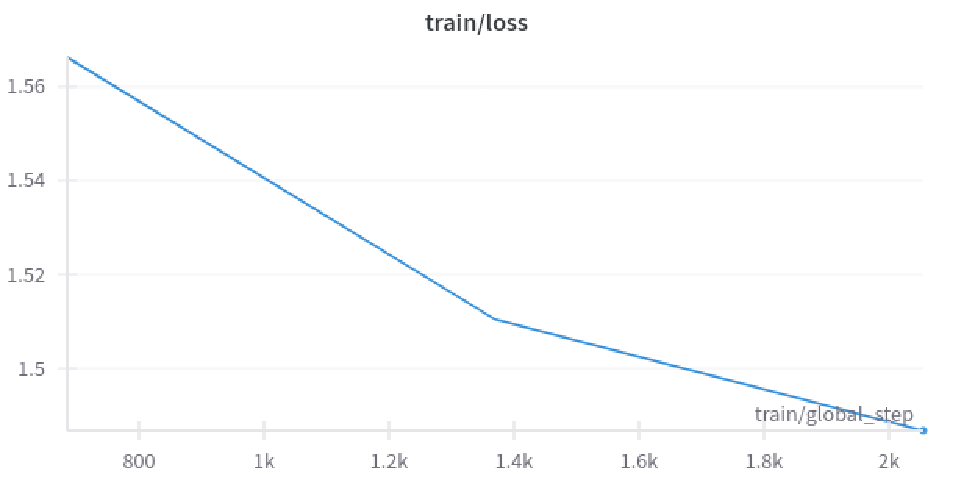
\includegraphics[width= \columnwidth]{figures/pred_only_sft_llama2_checkpoint-3000_train.pdf} 
%     \caption{Training loss progression for the \namel model during the Supervised Fine-Tuning (SFT) phase, focused solely on prediction tasks, using the LLaMa-2 architecture at checkpoint 3,000.}
%     \label{fig:sft_pred_train} % For referencing the figure
% \end{figure}
%%%%%%%%%%%%%%%%%%%%%%%%%%%%%%%%%%%%

%%%%%%%%%%%%%%%%%%%%%%%%%%%%%%%%%%%%
% \begin{figure}[ht] % [h] specifies the placement of the figure
%     \centering % Centers the figure
%     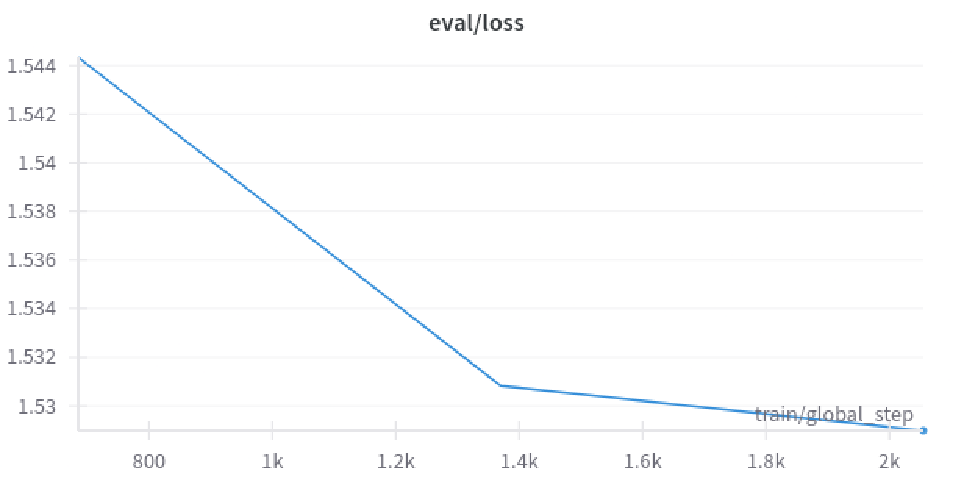
\includegraphics[width= \columnwidth]{figures/pred_only_sft_llama2_checkpoint-3000_eval.pdf} 
%     \caption{Evaluation loss progression for the \namel model during the Supervised Fine-Tuning (SFT) phase, focused solely on prediction tasks, using the LLaMa-2 architecture at checkpoint 3,000.}
%     \label{fig:sft_pred_val} % For referencing the figure
% \end{figure}
%%%%%%%%%%%%%%%%%%%%%%%%%%%%%%%%%%%%

%%%%%%%%%%%%%%%%%%%%%%%%%%%%%%%%%%%%
% \begin{figure}[ht] % [h] specifies the placement of the figure
%     \centering % Centers the figure
%     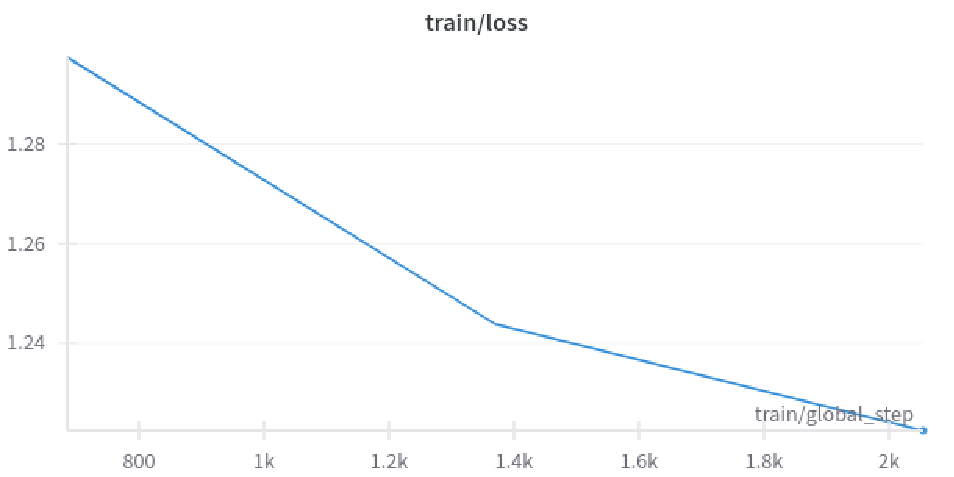
\includegraphics[width= \columnwidth]{figures/pred+expl_sft_for_1000_inp_500_op_model_train.pdf} 
%     \caption{Training loss progression for the \namel model during the Supervised Fine-Tuning (SFT) phase, focused on both prediction and explanation tasks, using the model setup for 1,000 input tokens and 500 output tokens.}
%     \label{fig:sft_pred_expl_train} % For referencing the figure
% \end{figure}
% %%%%%%%%%%%%%%%%%%%%%%%%%%%%%%%%%%%%

%%%%%%%%%%%%%%%%%%%%%%%%%%%%%%%%%%%%
% \begin{figure}[ht] % [h] specifies the placement of the figure
%     \centering % Centers the figure
%     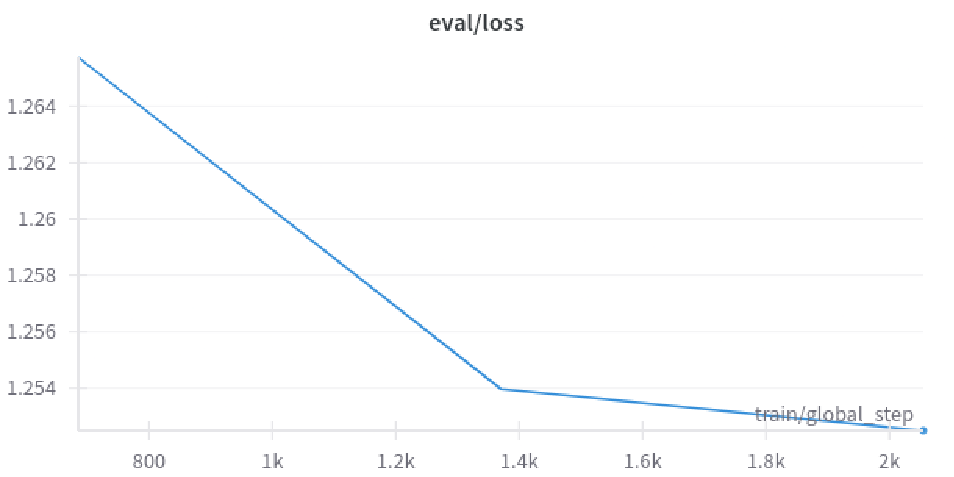
\includegraphics[width= \columnwidth]{figures/pred+expl_sft_for_1000_inp_500_op_model_eval.pdf} 
%     \caption{Evaluation loss progression for the \namel model during the Supervised Fine-Tuning (SFT) phase, focusing on both prediction and explanation tasks, using the model setup for 1,000 input tokens and 500 output tokens.}
%     \label{fig:sft_pred_expl_val} % For referencing the figure
% \end{figure}
%%%%%%%%%%%%%%%%%%%%%%%%%%%%%%%%%%%%


%%%%%%%%%%%%%%%%%%%%%%%%%%%%%%%%%%%%%%%%%%%%%%%
%  Binary-single-transformers
%%%%%%%%%%%%%%%%%%%%%%%%%%%%%%%%%%%%%%%%%%%%%%%
\begin{table}[t]
\centering
\resizebox{\columnwidth}{!}{%
\begin{tabular}{lrrrr}
\hline
\multicolumn{1}{l}{\textbf{Test Data}} &
  \multicolumn{1}{r}{\textbf{\begin{tabular}[c]{@{}c@{}}Macro \\ Precision\end{tabular}}} &
  \multicolumn{1}{r}{\textbf{\begin{tabular}[c]{@{}c@{}}Macro \\ Recall\end{tabular}}} &
  \multicolumn{1}{r}{\textbf{\begin{tabular}[c]{@{}c@{}}Macro \\ F1\end{tabular}}} &
  \multicolumn{1}{r}{\textbf{Accuracy}} \\ \hline
\multicolumn{5}{c}{\textbf{InLegalBert}}                                                                                                                              \\ \hline
ILDC                                                                                          & 0.7486          & 0.7464          & 0.7475          & 0.7462          \\
SCI (2019)                                                                                    & 0.8391          & 0.8391          & 0.8391          & 0.8388          \\
SCI (2020-24)                                                                                 & 0.8712          & 0.8875          & 0.8793          & 0.8913          \\
SCI+HCs (2019)                                                                                & 0.8843          & 0.8831          & 0.8837          & 0.8837          \\
HCs (2020-24)                                                                                 & \textbf{0.9006} & \textbf{0.9018} & \textbf{0.9012} & \textbf{0.9012} \\
SCI+HCs+Tribunal (2019)                                                                       & 0.8753          & 0.8749          & 0.8751          & 0.8751          \\
Tribunal (2020-24)                                                                            & 0.8545          & 0.8527          & 0.8536          & 0.8541          \\
\begin{tabular}[c]{@{}l@{}}SCI+HCs+Tribunal+\\ DailyOrders+DistrictCourts (2019)\end{tabular} & 0.8800          & 0.8795          & 0.8797          & 0.8797          \\
Daily\_orders (2020-24)                                                                       & 0.8734          & 0.8801          & 0.8768          & 0.8830          \\ \hline
\multicolumn{5}{c}{\textbf{InCaseLaw}}                                                                                                                                \\ \hline
ILDC                                                                                          & 0.7090          & 0.7085          & 0.7088          & 0.7086          \\
SCI (2019)                                                                                    & 0.8209          & 0.8209          & 0.8209          & 0.8209          \\
SCI (2020-24)                                                                                 & 0.8453          & 0.8659          & 0.8555          & 0.8681          \\
SCI+HCs (2019)                                                                                & 0.8564          & 0.8543          & 0.8554          & 0.8554          \\
HCs (2020-24)                                                                                 & \textbf{0.8708} & \textbf{0.8717} & \textbf{0.8712} & \textbf{0.8690} \\
SCI+HCs+Tribunal (2019)                                                                       & 0.8603          & 0.8593          & 0.8598          & 0.8596          \\
Tribunal (2020-24)                                                                            & 0.8451          & 0.8412          & 0.8431          & 0.8433          \\
\begin{tabular}[c]{@{}l@{}}SCI+HCs+Tribunal+\\ DailyOrders+DistrictCourts (2019)\end{tabular} & 0.8578          & 0.8565          & 0.8571          & 0.8570          \\
Daily\_orders (2020-24)                                                                       & 0.8457          & 0.8609          & 0.8532          & 0.8564          \\ \hline
\multicolumn{5}{c}{\textbf{XLNet Large}}                                                                                                                              \\ \hline
ILDC                                                                                          & 0.7112          & 0.7044          & 0.7078          & 0.7040          \\
SCI (2019)                                                                                    & 0.8095          & 0.8082          & 0.8089          & 0.8076          \\
SCI (2020-24)                                                                                 & 0.8255          & 0.8570          & 0.8410          & 0.8482          \\
SCI+HCs (2019)                                                                                & 0.8583          & 0.8533          & 0.8558          & 0.8550          \\
HCs (2020-24)                                                                                 & \textbf{0.8725} & \textbf{0.8724} & \textbf{0.8724} & \textbf{0.8688} \\
SCI+HCs+Tribunal (2019)                                                                       & 0.8653          & 0.8624          & 0.8639          & 0.8629          \\
Tribunal (2020-24)                                                                            & 0.8625          & 0.8570          & 0.8598          & 0.8595          \\
\begin{tabular}[c]{@{}l@{}}SCI+HCs+Tribunal+\\ DailyOrders+DistrictCourts (2019)\end{tabular} & 0.8640          & 0.8601          & 0.8620          & 0.8610          \\
Daily\_orders (2020-24)                                                                       & 0.8282          & 0.8473          & 0.8376          & 0.8363          \\ \hline
\end{tabular}%
}
\caption{Judgment prediction results on the binary task across different court cases and temporal test cases, with models trained on SCI + HCs + Tribunal data from \texttt{\named} single-split data. The best results are highlighted in bold.}
\label{tab:binary-judgment-results-single-SCI-HCs-Tribunal}
\end{table}
%%%%%%%%%%%%%%%%%%%%%%%%%%%%%%%%%%%%%%%%%%%%%%%
%%%%%%%%%%%%%%%%%%%%%%%%%%%%%%%%%%%%%%%%%%%%%%%
%  Binary-multi-transformers
%%%%%%%%%%%%%%%%%%%%%%%%%%%%%%%%%%%%%%%%%%%%%%%
\begin{table}[ht]
\centering
\resizebox{\columnwidth}{!}{%
\begin{tabular}{lrrrr}
 \hline
\multicolumn{1}{l}{\textbf{Test Data}} &
  \multicolumn{1}{r}{\textbf{\begin{tabular}[c]{@{}c@{}}Macro \\ Precision\end{tabular}}} &
  \multicolumn{1}{r}{\textbf{\begin{tabular}[c]{@{}c@{}}Macro \\ Recall\end{tabular}}} &
  \multicolumn{1}{r}{\textbf{\begin{tabular}[c]{@{}c@{}}Macro \\ F1\end{tabular}}} &
  \multicolumn{1}{r}{\textbf{Accuracy}} \\ \hline
\multicolumn{5}{c}{\textbf{InLegalBert}}                                                                                                                              \\ \hline
ILDC                                                                                          & 0.7209          & 0.7169          & 0.7189          & 0.7172          \\
SCI (2019)                                                                                    & 0.8261          & 0.8255          & 0.8258          & 0.8258          \\
SCI (2020-24)                                                                                 & 0.8515          & 0.8588          & 0.8552          & 0.8720          \\
SCI+HCs (2019)                                                                                & 0.8739          & 0.8735          & 0.8737          & 0.8739          \\
HCs (2020-24)                                                                                 & \textbf{0.8940} & \textbf{0.8943} & \textbf{0.8942} & 0.8945          \\
SCI+HCs+Tribunal (2019)                                                                       & 0.8637          & 0.8634          & 0.8635          & 0.8635          \\
Tribunal (2020-24)                                                                            & 0.8308          & 0.8249          & 0.8278          & 0.8277          \\
\begin{tabular}[c]{@{}l@{}}SCI+HCs+Tribunal+\\ DailyOrders+DistrictCourts (2019)\end{tabular} & 0.8722          & 0.8718          & 0.8720          & 0.8720          \\
Daily\_orders (2020-24)                                                                       & 0.8897          & 0.8869          & 0.8883          & \textbf{0.8955} \\ \hline
\multicolumn{5}{c}{\textbf{InCaseLaw}}                                                                                                                                \\ \hline
ILDC                                                                                          & 0.7347          & 0.7335          & 0.7341          & 0.7337          \\
SCI (2019)                                                                                    & 0.8271          & 0.8272          & 0.8271          & 0.8272          \\
SCI (2020-24)                                                                                 & 0.8449          & 0.8579          & 0.8513          & 0.8670          \\
SCI+HCs (2019)                                                                                & 0.8585          & 0.8570          & 0.8578          & 0.8579          \\
HCs (2020-24)                                                                                 & \textbf{0.8891} & \textbf{0.8898} & \textbf{0.8895} & 0.8898          \\
SCI+HCs+Tribunal (2019)                                                                       & 0.8544          & 0.8521          & 0.8532          & 0.8526          \\
Tribunal (2020-24)                                                                            & 0.8160          & 0.7939          & 0.8048          & 0.8001          \\
\begin{tabular}[c]{@{}l@{}}SCI+HCs+Tribunal+\\ DailyOrders+DistrictCourts (2019)\end{tabular} & 0.8573          & 0.8553          & 0.8563          & 0.8559          \\
Daily\_orders (2020-24)                                                                       & 0.8868          & 0.8795          & 0.8831          & \textbf{0.8911} \\ \hline
\multicolumn{5}{c}{\textbf{XLNet Large}}                                                                                                                              \\ \hline
ILDC                                                                                          & 0.6851          & 0.6850          & 0.6851          & 0.6849          \\
SCI (2019)                                                                                    & 0.8150          & 0.8137          & 0.8143          & 0.8142          \\
SCI (2020-24)                                                                                 & 0.8507          & 0.8562          & 0.8535          & 0.8709          \\
SCI+HCs (2019)                                                                                & 0.8590          & 0.8585          & 0.8588          & 0.8590          \\
HCs (2020-24)                                                                                 & \textbf{0.8848} & 0.8863          & 0.8856          & \textbf{0.8851} \\ 
SCI+HCs+Tribunal (2019)                                                                       & 0.8580          & 0.8576          & 0.8578          & 0.8577          \\
Tribunal (2020-24)                                                                            & 0.8180          & 0.8053          & 0.8116          & 0.8098          \\ 
\begin{tabular}[c]{@{}l@{}}SCI+HCs+Tribunal+\\ DailyOrders+DistrictCourts (2019)\end{tabular} & 0.8660          & 0.8655          & 0.8657          & 0.8657          \\
Daily\_orders (2020-24)                                                                       & 0.8832          & \textbf{0.8904} & \textbf{0.8868} & 0.8924       \\   \hline
\end{tabular}%
}
\caption{Judgment prediction results on the binary task across different court cases and temporal test cases, with models trained on SCI + HCs + Tribunal + Daily Orders and District Court data from \texttt{\named} multi-split data. The best results are highlighted in bold.}
\label{tab:binary-judgment-results-multi}
\end{table}

%%%%%%%%%%%%%%%%%%%%%%%%%%%%%%%%%%%%%%%%%%%%%%%

%%%%%%%%%%%%%%%%%%%%%%%%%%%%%%%%%%%%%%%%%%%%%%%
%  Binary Multi SCI+HCs+Tribunal
%%%%%%%%%%%%%%%%%%%%%%%%%%%%%%%%%%%%%%%%%%%%%%%
\begin{table}[t]
\centering
\resizebox{\columnwidth}{!}{%
\begin{tabular}{lrrrr}
\hline
\multicolumn{1}{l}{\textbf{Test Data}} &
  \multicolumn{1}{r}{\textbf{\begin{tabular}[c]{@{}c@{}}Macro \\ Precision\end{tabular}}} &
  \multicolumn{1}{r}{\textbf{\begin{tabular}[c]{@{}c@{}}Macro \\ Recall\end{tabular}}} &
  \multicolumn{1}{r}{\textbf{\begin{tabular}[c]{@{}c@{}}Macro \\ F1\end{tabular}}} &
  \multicolumn{1}{r}{\textbf{Accuracy}} \\ \hline
\multicolumn{5}{c}{\textbf{InLegalBert}}                                                                                                                              \\ \hline
ILDC                                                                                          & 0.7492          & 0.7351          & 0.7421          & 0.7357          \\
SCI (2019)                                                                                    & 0.8532          & 0.8437          & 0.8484          & 0.8451          \\
SCI (2020-24)                                                                                 & \textbf{0.9102} & 0.8798          & \textbf{0.8947} & \textbf{0.9095} \\
SCI+HCs (2019)                                                                                & 0.8822          & 0.8814          & 0.8818          & 0.8799          \\
HCs (2020-24)                                                                                 & 0.8908          & \textbf{0.8869} & 0.8888          & 0.8891          \\
SCI+HCs+Tribunal (2019)                                                                       & 0.8785          & 0.8744          & 0.8764          & 0.8737          \\
Tribunal (2020-24)                                                                            & 0.8275          & 0.8194          & 0.8234          & 0.8142          \\
\begin{tabular}[c]{@{}l@{}}SCI+HCs+Tribunal+\\ DailyOrders+DistrictCourts (2019)\end{tabular} & 0.8544          & 0.8493          & 0.8519          & 0.8483          \\
Daily\_orders (2020-24)                                                                       & 0.8852          & 0.8686          & 0.8768          & 0.8855          \\ \hline
\multicolumn{5}{c}{\textbf{InCaseLaw}}                                                                                                                                \\ \hline
ILDC                                                                                          & 0.6856          & 0.6369          & 0.6604          & 0.6381          \\
SCI (2019)                                                                                    & 0.7965          & 0.7744          & 0.7852          & 0.7767          \\
SCI (2020-24)                                                                                 & \textbf{0.8673} & 0.8385          & \textbf{0.8526} & \textbf{0.8742} \\
SCI+HCs (2019)                                                                                & 0.8211          & 0.8152          & 0.8182          & 0.8124          \\
HCs (2020-24)                                                                                 & 0.8501          & \textbf{0.8446} & 0.8474          & 0.8477          \\
SCI+HCs+Tribunal (2019)                                                                       & 0.8262          & 0.8164          & 0.8213          & 0.8153          \\
Tribunal (2020-24)                                                                            & 0.8234          & 0.8194          & 0.8214          & 0.8154          \\
\begin{tabular}[c]{@{}l@{}}SCI+HCs+Tribunal+\\ DailyOrders+DistrictCourts (2019)\end{tabular} & 0.8259          & 0.8174          & 0.8216          & 0.8157          \\
Daily\_orders (2020-24)                                                                       & 0.8624          & 0.8379          & 0.8500          & 0.8610          \\ \hline
\multicolumn{5}{c}{\textbf{XLNet Large}}                                                                                                                              \\ \hline
ILDC                                                                                          & 0.7257          & 0.7107          & 0.7181          & 0.7113          \\
SCI (2019)                                                                                    & 0.8479          & 0.8356          & 0.8417          & 0.8371          \\
SCI (2020-24)                                                                                 & 0.8965          & 0.8794          & 0.8878          & 0.9034          \\
SCI+HCs (2019)                                                                                & 0.8686          & 0.8668          & 0.8677          & 0.8650          \\
HCs (2020-24)                                                                                 & \textbf{0.9065} & \textbf{0.9023} & \textbf{0.9044} & \textbf{0.9045} \\
SCI+HCs+Tribunal (2019)                                                                       & 0.8634          & 0.8571          & 0.8602          & 0.8562          \\
Tribunal (2020-24)                                                                            & 0.8255          & 0.8198          & 0.8227          & 0.8153          \\
\begin{tabular}[c]{@{}l@{}}SCI+HCs+Tribunal+\\ DailyOrders+DistrictCourts (2019)\end{tabular} & 0.8613          & 0.8557          & 0.8585          & 0.8544          \\
Daily\_orders (2020-24)                                                                       & 0.8813          & 0.8638          & 0.8725          & 0.8815          \\ \hline
\end{tabular}%
}
\caption{Judgment prediction results on the binary task across different court cases and temporal test cases, with models trained on SCI + HCs + Tribunal data from \texttt{\named} multi-split data. The best results are highlighted in bold.}
\label{tab:binary-judgment-results-multi-SCI-HCs-Tribunal}
\end{table}
%%%%%%%%%%%%%%%%%%%%%%%%%%%%%%%%%%%%%%%%%%%%%%%

%%%%%%%%%%%%%%%%%%%%%%%%%%%%%%%%%%%%%%%%%%%%%%%
%  Binary Single SCI+HCs
%%%%%%%%%%%%%%%%%%%%%%%%%%%%%%%%%%%%%%%%%%%%%%%
\begin{table}[t]
\centering
\resizebox{\columnwidth}{!}{%
\begin{tabular}{lrrrr}
\hline
\multicolumn{1}{l}{\textbf{Test Data}} &
  \multicolumn{1}{r}{\textbf{\begin{tabular}[c]{@{}c@{}}Macro \\ Precision\end{tabular}}} &
  \multicolumn{1}{r}{\textbf{\begin{tabular}[c]{@{}c@{}}Macro \\ Recall\end{tabular}}} &
  \multicolumn{1}{r}{\textbf{\begin{tabular}[c]{@{}c@{}}Macro \\ F1\end{tabular}}} &
  \multicolumn{1}{r}{\textbf{Accuracy}} \\ \hline
\multicolumn{5}{c}{\textbf{InLegalBert}}                                                                                                                              \\ \hline
ILDC                                                                                          & 0.7544          & 0.7536          & 0.7540          & 0.7535          \\
SCI (2019)                                                                                    & 0.8309          & 0.8308          & 0.8308          & 0.8309          \\
SCI (2020-24)                                                                                 & 0.8742          & 0.8807          & 0.8774          & 0.8918          \\
SCI+HCs (2019)                                                                                & 0.8691          & 0.8692          & 0.8692          & 0.8693          \\
HCs (2020-24)                                                                                 & \textbf{0.8952} & \textbf{0.8953} & \textbf{0.8952} & \textbf{0.8956} \\
SCI+HCs+Tribunal (2019)                                                                       & 0.8542          & 0.8538          & 0.8540          & 0.8540          \\
Tribunal (2020-24)                                                                            & 0.8086          & 0.7849          & 0.7966          & 0.7914          \\
\begin{tabular}[c]{@{}l@{}}SCI+HCs+Tribunal+\\ DailyOrders+DistrictCourts (2019)\end{tabular} & 0.7499          & 0.7421          & 0.7460          & 0.7406          \\
Daily\_orders (2020-24)                                                                       & 0.8687          & 0.8684          & 0.8685          & 0.8767          \\ \hline
\multicolumn{5}{c}{\textbf{InCaseLaw}}                                                                                                                                \\ \hline
ILDC                                                                                          & 0.7513          & 0.7503          & 0.7508          & 0.7502          \\
SCI (2019)                                                                                    & 0.8327          & 0.8328          & 0.8328          & 0.8327          \\
SCI (2020-24)                                                                                 & 0.8555          & 0.8710          & 0.8632          & 0.8769          \\
SCI+HCs (2019)                                                                                & 0.8660          & 0.8652          & 0.8656          & 0.8658          \\
HCs (2020-24)                                                                                 & \textbf{0.8961} & \textbf{0.8969} & \textbf{0.8965} & \textbf{0.8967} \\
SCI+HCs+Tribunal (2019)                                                                       & 0.8511          & 0.8494          & 0.8503          & 0.8498          \\
Tribunal (2020-24)                                                                            & 0.7923          & 0.7599          & 0.7758          & 0.7679          \\
\begin{tabular}[c]{@{}l@{}}SCI+HCs+Tribunal+\\ DailyOrders+DistrictCourts (2019)\end{tabular} & 0.8497          & 0.8479          & 0.8488          & 0.8485          \\
Daily\_orders (2020-24)                                                                       & 0.8696          & 0.8721          & 0.8709          & 0.8784          \\ \hline
\multicolumn{5}{c}{\textbf{XLNet Large}}                                                                                                                              \\ \hline
ILDC                                                                                          & 0.7247          & 0.7245          & 0.7246          & 0.7245          \\
SCI (2019)                                                                                    & 0.8375          & 0.8368          & 0.8372          & 0.8371          \\
SCI (2020-24)                                                                                 & 0.8680          & 0.8792          & 0.8736          & 0.8874          \\
SCI+HCs (2019)                                                                                & 0.8788          & 0.8792          & 0.8790          & 0.8789          \\
HCs (2020-24)                                                                                 & \textbf{0.9101} & \textbf{0.9099} & \textbf{0.9100} & \textbf{0.9104} \\
SCI+HCs+Tribunal (2019)                                                                       & 0.8649          & 0.8650          & 0.8649          & 0.8649          \\
Tribunal (2020-24)                                                                            & 0.8114          & 0.8008          & 0.8060          & 0.8049          \\
\begin{tabular}[c]{@{}l@{}}SCI+HCs+Tribunal+\\ DailyOrders+DistrictCourts (2019)\end{tabular} & 0.8653          & 0.8654          & 0.8654          & 0.8654          \\
Daily\_orders (2020-24)                                                                       & 0.8684          & 0.8741          & 0.8713          & 0.8780          \\ \hline
\end{tabular}%
}
\caption{Judgment prediction results on the binary task across different court cases and temporal test cases, with models trained on SCI + HCs data from \texttt{\named} single split data. The best results are highlighted in bold.}
\label{tab:binary-judgment-results-single-SCI-HCs}
\end{table}
%%%%%%%%%%%%%%%%%%%%%%%%%%%%%%%%%%%%%%%%%%%%%%%

%%%%%%%%%%%%%%%%%%%%%%%%%%%%%%%%%%%%%%%%%%%%%%%
%  Binary Multi SCI+HCs
%%%%%%%%%%%%%%%%%%%%%%%%%%%%%%%%%%%%%%%%%%%%%%%
\begin{table}[t]
\centering
\resizebox{\columnwidth}{!}{%
\begin{tabular}{lrrrr}
\hline
\multicolumn{1}{l}{\textbf{Test Data}} &
  \multicolumn{1}{r}{\textbf{\begin{tabular}[c]{@{}c@{}}Macro \\ Precision\end{tabular}}} &
  \multicolumn{1}{r}{\textbf{\begin{tabular}[c]{@{}c@{}}Macro \\ Recall\end{tabular}}} &
  \multicolumn{1}{r}{\textbf{\begin{tabular}[c]{@{}c@{}}Macro \\ F1\end{tabular}}} &
  \multicolumn{1}{r}{\textbf{Accuracy}} \\ \hline
\multicolumn{5}{c}{\textbf{InLegalBert}}                                                                                                                              \\ \hline
ILDC                                                                                          & 0.7364          & 0.7078          & 0.7218          & 0.7086          \\
SCI (2019)                                                                                    & 0.8480          & 0.8323          & 0.8401          & 0.8341          \\
SCI (2020-24)                                                                                 & 0.8986          & 0.8614          & 0.8796          & 0.8968          \\
SCI+HCs (2019)                                                                                & 0.8689          & 0.8653          & 0.8671          & 0.8630          \\
HCs (2020-24)                                                                                 & \textbf{0.8949} & \textbf{0.8881} & \textbf{0.8915} & \textbf{0.8912} \\
SCI+HCs+Tribunal (2019)                                                                       & 0.8529          & 0.8474          & 0.8501          & 0.8465          \\
Tribunal (2020-24)                                                                            & 0.8069          & 0.8072          & 0.8071          & 0.8074          \\
\begin{tabular}[c]{@{}l@{}}SCI+HCs+Tribunal+\\ DailyOrders+DistrictCourts (2019)\end{tabular} & 0.7672          & 0.7406          & 0.7537          & 0.7381          \\
Daily\_orders (2020-24)                                                                       & 0.8779          & 0.8593          & 0.8685          & 0.8779          \\ \hline
\multicolumn{5}{c}{\textbf{InCaseLaw}}                                                                                                                                \\ \hline
ILDC                                                                                          & 0.6963          & 0.6675          & 0.6816          & 0.6684          \\
SCI (2019)                                                                                    & 0.8062          & 0.7930          & 0.7995          & 0.7947          \\
SCI (2020-24)                                                                                 & 0.8652          & 0.8516          & 0.8584          & \textbf{0.8780} \\
SCI+HCs (2019)                                                                                & 0.8315          & 0.8265          & 0.8290          & 0.8239          \\
HCs (2020-24)                                                                                 & \textbf{0.8678} & \textbf{0.8584} & \textbf{0.8631} & 0.8624          \\
SCI+HCs+Tribunal (2019)                                                                       & 0.8174          & 0.8112          & 0.8143          & 0.8102          \\
Tribunal (2020-24)                                                                            & 0.7831          & 0.7828          & 0.7829          & 0.7836          \\
\begin{tabular}[c]{@{}l@{}}SCI+HCs+Tribunal+\\ DailyOrders+DistrictCourts (2019)\end{tabular} & 0.8172          & 0.8118          & 0.8145          & 0.8104          \\
Daily\_orders (2020-24)                                                                       & 0.8583          & 0.8304          & 0.8441          & 0.8555          \\ \hline
\multicolumn{5}{c}{\textbf{XLNet Large}}                                                                                                                              \\ \hline
ILDC                                                                                          & 0.7265          & 0.7181          & 0.7223          & 0.7185          \\
SCI (2019)                                                                                    & 0.8412          & 0.8292          & 0.8351          & 0.8307          \\
SCI (2020-24)                                                                                 & \textbf{0.9118} & 0.8910          & 0.9013          & \textbf{0.9150} \\
SCI+HCs (2019)                                                                                & 0.8645          & 0.8624          & 0.8635          & 0.8605          \\
HCs (2020-24)                                                                                 & 0.9060          & \textbf{0.9014} & \textbf{0.9037} & 0.9037          \\
SCI+HCs+Tribunal (2019)                                                                       & 0.8505          & 0.8466          & 0.8485          & 0.8459          \\
Tribunal (2020-24)                                                                            & 0.8159          & 0.8166          & 0.8162          & 0.8164          \\
\begin{tabular}[c]{@{}l@{}}SCI+HCs+Tribunal+\\ DailyOrders+DistrictCourts (2019)\end{tabular} & 0.8506          & 0.8471          & 0.8488          & 0.8462          \\
Daily\_orders (2020-24)                                                                       & 0.8783          & 0.8606          & 0.8693          & 0.8787          \\ \hline
\end{tabular}%
}
\caption{Judgment prediction results on the binary task across different court cases and temporal test cases, with models trained on SCI + HCs data from \texttt{\named} multi-split data. The best results are highlighted in bold.}
\label{tab:binary-judgment-results-multi-SCI-HCs}
\end{table}
%%%%%%%%%%%%%%%%%%%%%%%%%%%%%%%%%%%%%%%%%%%%%%%

%%%%%%%%%%%%%%%%%%%%%%%%%%%%%%%%%%%%%%%%%%%%%%%
%  Binary Single SCI
%%%%%%%%%%%%%%%%%%%%%%%%%%%%%%%%%%%%%%%%%%%%%%%
\begin{table}[t]
\centering
\resizebox{\columnwidth}{!}{%
\begin{tabular}{lrrrr}
\hline
\multicolumn{1}{l}{\textbf{Test Data}} &
  \multicolumn{1}{r}{\textbf{\begin{tabular}[c]{@{}c@{}}Macro \\ Precision\end{tabular}}} &
  \multicolumn{1}{r}{\textbf{\begin{tabular}[c]{@{}c@{}}Macro \\ Recall\end{tabular}}} &
  \multicolumn{1}{r}{\textbf{\begin{tabular}[c]{@{}c@{}}Macro \\ F1\end{tabular}}} &
  \multicolumn{1}{r}{\textbf{Accuracy}} \\ \hline
\multicolumn{5}{c}{\textbf{InLegalBert}}                                                                                                                              \\ \hline
ILDC                                                                                          & 0.7147          & 0.7145          & 0.7146          & 0.7146          \\
SCI (2019)                                                                                    & 0.8212          & 0.8187          & 0.8200          & 0.8194          \\
SCI (2020-24)                                                                                 & \textbf{0.8983} & \textbf{0.8532} & \textbf{0.8752} & \textbf{0.8929}  \\
SCI+HCs (2019)                                                                                & 0.7691          & 0.7664          & 0.7677          & 0.7642          \\
HCs (2020-24)                                                                                 & 0.7919          & 0.7585          & 0.7748          & 0.7683          \\
SCI+HCs+Tribunal (2019)                                                                       & 0.7514          & 0.7447          & 0.7481          & 0.7437          \\
Tribunal (2020-24)                                                                            & 0.7300          & 0.6655          & 0.6963          & 0.6514          \\
\begin{tabular}[c]{@{}l@{}}SCI+HCs+Tribunal+\\ DailyOrders+DistrictCourts (2019)\end{tabular} & 0.7499          & 0.7421          & 0.7460          & 0.7406          \\
Daily\_orders (2020-24)                                                                       & 0.7849          & 0.7389          & 0.7612          & 0.7814          \\ \hline
\multicolumn{5}{c}{\textbf{InCaseLaw}}                                                                                                                                \\ \hline
ILDC                                                                                          & 0.7067          & 0.7066          & 0.7066          & 0.7067          \\
SCI (2019)                                                                                    & 0.8093          & 0.8083          & 0.8088          & 0.8088          \\
SCI (2020-24)                                                                                 & \textbf{0.8782} & 0.8394          & 0.8584          & \textbf{0.8791} \\
SCI+HCs (2019)                                                                                & 0.7596          & 0.7578          & 0.7587          & 0.7559          \\
HCs (2020-24)                                                                                 & 0.8678          & \textbf{0.8584} & \textbf{0.8631} & 0.8624          \\
SCI+HCs+Tribunal (2019)                                                                       & 0.7420          & 0.7369          & 0.7394          & 0.7359          \\
Tribunal (2020-24)                                                                            & 0.7031          & 0.6493          & 0.6751          & 0.6355          \\
\begin{tabular}[c]{@{}l@{}}SCI+HCs+Tribunal+\\ DailyOrders+DistrictCourts (2019)\end{tabular} & 0.7397          & 0.7340          & 0.7368          & 0.7324          \\
Daily\_orders (2020-24)                                                                       & 0.7826          & 0.7356          & 0.7584          & 0.7790          \\ \hline
\multicolumn{5}{c}{\textbf{XLNet Large}}                                                                                                                              \\ \hline
ILDC                                                                                          & 0.7356          & 0.7342          & 0.7349          & 0.7343          \\
SCI (2019)                                                                                    & 0.8495          & 0.8488          & 0.8492          & 0.8491          \\
SCI (2020-24)                                                                                 & \textbf{0.9185} & \textbf{0.8961} & \textbf{0.9071} & \textbf{0.9200} \\
SCI+HCs (2019)                                                                                & 0.8064          & 0.8063          & 0.8063          & 0.8052          \\
HCs (2020-24)                                                                                 & 0.8342          & 0.8288          & 0.8315          & 0.8320          \\
SCI+HCs+Tribunal (2019)                                                                       & 0.7936          & 0.7912          & 0.7924          & 0.7906          \\
Tribunal (2020-24)                                                                            & 0.7810          & 0.7629          & 0.7718          & 0.7555          \\
\begin{tabular}[c]{@{}l@{}}SCI+HCs+Tribunal+\\ DailyOrders+DistrictCourts (2019)\end{tabular} & 0.7916          & 0.7894          & 0.7905          & 0.7887          \\
Daily\_orders (2020-24)                                                                       & 0.8224          & 0.8167          & 0.8195          & 0.8319          \\ \hline
\end{tabular}%
}
\caption{Judgment prediction results on the binary task across different court cases and temporal test cases, with models trained on SCI data from \texttt{\named} single split data. The best results are highlighted in bold.}
\label{tab:binary-judgment-results-single-SCI}
\end{table}
%%%%%%%%%%%%%%%%%%%%%%%%%%%%%%%%%%%%%%%%%%%%%%%


%%%%%%%%%%%%%%%%%%%%%%%%%%%%%%%%%%%%%%%%%%%%%%%
%  Binary Multi SCI
%%%%%%%%%%%%%%%%%%%%%%%%%%%%%%%%%%%%%%%%%%%%%%%
\begin{table}[t]
\centering
\resizebox{\columnwidth}{!}{%
\begin{tabular}{lrrrr}
\hline
\multicolumn{1}{l}{\textbf{Test Data}} &
  \multicolumn{1}{r}{\textbf{\begin{tabular}[c]{@{}c@{}}Macro \\ Precision\end{tabular}}} &
  \multicolumn{1}{r}{\textbf{\begin{tabular}[c]{@{}c@{}}Macro \\ Recall\end{tabular}}} &
  \multicolumn{1}{r}{\textbf{\begin{tabular}[c]{@{}c@{}}Macro \\ F1\end{tabular}}} &
  \multicolumn{1}{r}{\textbf{Accuracy}} \\ \hline
\multicolumn{5}{c}{\textbf{InLegalBert}}                                                                                                                              \\ \hline
ILDC                                                                                          & 0.7216          & 0.6866          & 0.7037          & 0.6875          \\
SCI (2019)                                                                                    & 0.8370          & 0.8230          & 0.8299          & 0.8246          \\
SCI (2020-24)                                                                                 & \textbf{0.9107} & \textbf{0.8546} & \textbf{0.8818} & \textbf{0.8979} \\
SCI+HCs (2019)                                                                                & 0.7781          & 0.7623          & 0.7701          & 0.7577          \\
HCs (2020-24)                                                                                 & 0.8051          & 0.7709          & 0.7876          & 0.7806          \\
SCI+HCs+Tribunal (2019)                                                                       & 0.7678          & 0.7427          & 0.7550          & 0.7407          \\
Tribunal (2020-24)                                                                            & 0.7354          & 0.6537          & 0.6921          & 0.6380          \\
\begin{tabular}[c]{@{}l@{}}SCI+HCs+Tribunal+\\ DailyOrders+DistrictCourts (2019)\end{tabular} & 0.7672          & 0.7406          & 0.7537          & 0.7381          \\
Daily\_orders (2020-24)                                                                       & 0.8241          & 0.7509          & 0.7858          & 0.8003          \\ \hline
\multicolumn{5}{c}{\textbf{InCaseLaw}}                                                                                                                                \\ \hline
ILDC                                                                                          & 0.7134          & 0.6881          & 0.7005          & 0.6889          \\
SCI (2019)                                                                                    & 0.8385          & 0.8265          & 0.8325          & 0.8280          \\
SCI (2020-24)                                                                                 & \textbf{0.9042} & 0.8535          & \textbf{0.8781} & \textbf{0.8951} \\
SCI+HCs (2019)                                                                                & 0.7696          & 0.7546          & 0.7620          & 0.7501          \\
HCs (2020-24)                                                                                 & 0.8678          & \textbf{0.8584} & 0.8631          & 0.8624          \\
SCI+HCs+Tribunal (2019)                                                                       & 0.7631          & 0.7391          & 0.7509          & 0.7371          \\
Tribunal (2020-24)                                                                            & 0.7272          & 0.6485          & 0.6856          & 0.6328          \\
\begin{tabular}[c]{@{}l@{}}SCI+HCs+Tribunal+\\ DailyOrders+DistrictCourts (2019)\end{tabular} & 0.7607          & 0.7367          & 0.7485          & 0.7337          \\
Daily\_orders (2020-24)                                                                       & 0.8140          & 0.7386          & 0.7744          & 0.7903          \\ \hline
\multicolumn{5}{c}{\textbf{XLNet Large}}                                                                                                                              \\ \hline
ILDC                                                                                          & 0.7229          & 0.7020          & 0.7123          & 0.7027          \\
SCI (2019)                                                                                    & 0.8851          & 0.8776          & 0.8813          & 0.8787          \\
SCI (2020-24)                                                                                 & \textbf{0.9187} & \textbf{0.8787} & \textbf{0.8982} & \textbf{0.9123} \\
SCI+HCs (2019)                                                                                & 0.8026          & 0.7921          & 0.7973          & 0.7884          \\
HCs (2020-24)                                                                                 & 0.8282          & 0.8097          & 0.8189          & 0.8162          \\
SCI+HCs+Tribunal (2019)                                                                       & 0.7913          & 0.7726          & 0.7818          & 0.7710          \\
Tribunal (2020-24)                                                                            & 0.7748          & 0.7402          & 0.7571          & 0.7303          \\
\begin{tabular}[c]{@{}l@{}}SCI+HCs+Tribunal+\\ DailyOrders+DistrictCourts (2019)\end{tabular} & 0.7901          & 0.7717          & 0.7808          & 0.7697          \\
Daily\_orders (2020-24)                                                                       & 0.8300          & 0.7825          & 0.8056          & 0.8201          \\ \hline
\end{tabular}%
}
\caption{Judgment prediction results on the binary task across different court cases and temporal test cases, with models trained on SCI data from \texttt{\named} multi-split data. The best results are highlighted in bold.}
\label{tab:binary-judgment-results-multi-SCI}
\end{table}
%%%%%%%%%%%%%%%%%%%%%%%%%%%%%%%%%%%%%%%%%%%%%%%

%%%%%%%%%%%%%%%%%%%%%%%%%%%%%%%%%%%%%%%%%%%%%%%
%  Binary ILDC Single
%%%%%%%%%%%%%%%%%%%%%%%%%%%%%%%%%%%%%%%%%%%%%%%
\begin{table}[t]
\centering
\resizebox{\columnwidth}{!}{%
\begin{tabular}{lrrrr}
\hline
\multicolumn{1}{l}{\textbf{Test Data}} &
  \multicolumn{1}{r}{\textbf{\begin{tabular}[c]{@{}c@{}}Macro \\ Precision\end{tabular}}} &
  \multicolumn{1}{r}{\textbf{\begin{tabular}[c]{@{}c@{}}Macro \\ Recall\end{tabular}}} &
  \multicolumn{1}{r}{\textbf{\begin{tabular}[c]{@{}c@{}}Macro \\ F1\end{tabular}}} &
  \multicolumn{1}{r}{\textbf{Accuracy}} \\ \hline
\multicolumn{5}{c}{\textbf{InLegalBert}}                                                                                                                              \\ \hline
ILDC                                                                                          & 0.7447          & 0.7437          & 0.7442          & 0.7436          \\
SCI (2019)                                                                                    & 0.7559          & 0.7516          & 0.7538          & 0.7527          \\
SCI (2020-24)                                                                                 & \textbf{0.8259} & \textbf{0.7305} & \textbf{0.7753} & \textbf{0.8113} \\
SCI+HCs (2019)                                                                                & 0.6810          & 0.6657          & 0.6733          & 0.6604          \\
HCs (2020-24)                                                                                 & 0.6766          & 0.6155          & 0.6446          & 0.6338          \\
SCI+HCs+Tribunal (2019)                                                                       & 0.6562          & 0.6384          & 0.6472          & 0.6362          \\
Tribunal (2020-24)                                                                            & 0.6446          & 0.5566          & 0.5974          & 0.5363          \\
\begin{tabular}[c]{@{}l@{}}SCI+HCs+Tribunal+\\ DailyOrders+DistrictCourts (2019)\end{tabular} & 0.6793          & 0.6722          & 0.6757          & 0.6737          \\
Daily\_orders (2020-24)                                                                       & 0.6865          & 0.6033          & 0.6422          & 0.6829          \\ \hline
\multicolumn{5}{c}{\textbf{InCaseLaw}}                                                                                                                                \\ \hline
ILDC                                                                                          & 0.7451          & 0.7380          & 0.7415          & 0.7376          \\
SCI (2019)                                                                                    & 0.7367          & 0.7347          & 0.7357          & 0.7354          \\
SCI (2020-24)                                                                                 & \textbf{0.7876} & \textbf{0.6971} & \textbf{0.7396} & \textbf{0.7848} \\
SCI+HCs (2019)                                                                                & 0.6573          & 0.6460          & 0.6516          & 0.6411          \\
HCs (2020-24)                                                                                 & 0.6306          & 0.5864          & 0.6077          & 0.6046          \\
SCI+HCs+Tribunal (2019)                                                                       & 0.6341          & 0.6188          & 0.6264          & 0.6167          \\
Tribunal (2020-24)                                                                            & 0.6362          & 0.5480          & 0.5888          & 0.5271          \\
\begin{tabular}[c]{@{}l@{}}SCI+HCs+Tribunal+\\ DailyOrders+DistrictCourts (2019)\end{tabular} & 0.6333          & 0.6158          & 0.6244          & 0.6123          \\
Daily\_orders (2020-24)                                                                       & 0.6648          & 0.5959          & 0.6285          & 0.6736          \\ \hline
\multicolumn{5}{c}{\textbf{XLNet Large}}                                                                                                                              \\ \hline
ILDC                                                                                          & 0.7429          & 0.7361          & 0.7395          & 0.7357          \\
SCI (2019)                                                                                    & 0.7577          & 0.7575          & 0.7576          & 0.7577          \\
SCI (2020-24)                                                                                 & \textbf{0.7963} & \textbf{0.7855} & \textbf{0.7909} & \textbf{0.8201} \\
SCI+HCs (2019)                                                                                & 0.7114          & 0.7114          & 0.7114          & 0.7118          \\
HCs (2020-24)                                                                                 & 0.6982          & 0.6988          & 0.6985          & 0.6990          \\
SCI+HCs+Tribunal (2019)                                                                       & 0.6897          & 0.6897          & 0.6897          & 0.6897          \\
Tribunal (2020-24)                                                                            & 0.6613          & 0.6515          & 0.6564          & 0.6446          \\
\begin{tabular}[c]{@{}l@{}}SCI+HCs+Tribunal+\\ DailyOrders+DistrictCourts (2019)\end{tabular} & 0.6895          & 0.6895          & 0.6895          & 0.6894          \\
Daily\_orders (2020-24)                                                                       & 0.7028          & 0.7064          & 0.7046          & 0.7199          \\ \hline
\end{tabular}%
}
\caption{Judgment prediction results on the binary task across different court cases and temporal test cases, with models trained on data from ILDC single data. The best results are highlighted in bold.}
\label{tab:binary-judgment-results-ILDC-single}
\end{table}
%%%%%%%%%%%%%%%%%%%%%%%%%%%%%%%%%%%%%%%%%%%%%%%


%%%%%%%%%%%%%%%%%%%%%%%%%%%%%%%%%%%%%%%%%%%%%%%
%  Binary ILDC Multi
%%%%%%%%%%%%%%%%%%%%%%%%%%%%%%%%%%%%%%%%%%%%%%%
\begin{table}[t]
\centering
\resizebox{\columnwidth}{!}{%
\begin{tabular}{lrrrr}
\hline
\multicolumn{1}{l}{\textbf{Test Data}} &
  \multicolumn{1}{r}{\textbf{\begin{tabular}[c]{@{}c@{}}Macro \\ Precision\end{tabular}}} &
  \multicolumn{1}{r}{\textbf{\begin{tabular}[c]{@{}c@{}}Macro \\ Recall\end{tabular}}} &
  \multicolumn{1}{r}{\textbf{\begin{tabular}[c]{@{}c@{}}Macro \\ F1\end{tabular}}} &
  \multicolumn{1}{r}{\textbf{Accuracy}} \\ \hline
\multicolumn{5}{c}{\textbf{InLegalBert}}                                                                                                                              \\ \hline
ILDC                                                                                          & 0.7706          & 0.7650          & 0.7678          & 0.7647          \\
SCI (2019)                                                                                    & 0.7799          & 0.7735          & 0.7767          & 0.7721          \\
SCI (2020-24)                                                                                 & \textbf{0.7868} & \textbf{0.8231} & \textbf{0.8045} & \textbf{0.8046} \\
SCI+HCs (2019)                                                                                & 0.7035          & 0.6907          & 0.6971          & 0.6949          \\
HCs (2020-24)                                                                                 & 0.6551          & 0.6446          & 0.6498          & 0.6355          \\
SCI+HCs+Tribunal (2019)                                                                       & 0.6840          & 0.6770          & 0.6805          & 0.6782          \\
Tribunal (2020-24)                                                                            & 0.6463          & 0.6464          & 0.6463          & 0.6447          \\
\begin{tabular}[c]{@{}l@{}}SCI+HCs+Tribunal+\\ DailyOrders+DistrictCourts (2019)\end{tabular} & 0.6544          & 0.6337          & 0.6439          & 0.6308          \\
Daily\_orders (2020-24)                                                                       & 0.5982          & 0.5918          & 0.5950          & 0.5428          \\ \hline
\multicolumn{5}{c}{\textbf{InCaseLaw}}                                                                                                                                \\ \hline
ILDC                                                                                          & 0.7592          & 0.7461          & 0.7526          & 0.7456          \\
SCI (2019)                                                                                    & \textbf{0.7691} & 0.7622          & 0.7656          & 0.7608          \\
SCI (2020-24)                                                                                 & 0.7687          & \textbf{0.8068} & \textbf{0.7873} & \textbf{0.7765} \\
SCI+HCs (2019)                                                                                & 0.6908          & 0.6822          & 0.6865          & 0.6857          \\
HCs (2020-24)                                                                                 & 0.6367          & 0.6271          & 0.6319          & 0.6180          \\
SCI+HCs+Tribunal (2019)                                                                       & 0.6691          & 0.6651          & 0.6671          & 0.6661          \\
Tribunal (2020-24)                                                                            & 0.6242          & 0.6241          & 0.6242          & 0.6221          \\
\begin{tabular}[c]{@{}l@{}}SCI+HCs+Tribunal+\\ DailyOrders+DistrictCourts (2019)\end{tabular} & 0.6667          & 0.6628          & 0.6647          & 0.6642          \\
Daily\_orders (2020-24)                                                                       & 0.5842          & 0.5818          & 0.5830          & 0.5399          \\ \hline
\multicolumn{5}{c}{\textbf{XLNet Large}}                                                                                                                              \\ \hline
ILDC                                                                                          & 0.7873          & 0.7840          & 0.7856          & 0.7838          \\
SCI (2019)                                                                                    & \textbf{0.8104} & \textbf{0.7959} & \textbf{0.8031} & \textbf{0.7939} \\
SCI (2020-24)                                                                                 & 0.7483          & 0.7839          & 0.7657          & 0.7417          \\
SCI+HCs (2019)                                                                                & 0.7224          & 0.7023          & 0.7122          & 0.7074          \\
HCs (2020-24)                                                                                 & 0.6918          & 0.6677          & 0.6795          & 0.6556          \\
SCI+HCs+Tribunal (2019)                                                                       & 0.7100          & 0.6949          & 0.7023          & 0.6965          \\
Tribunal (2020-24)                                                                            & 0.6704          & 0.6559          & 0.6631          & 0.6631          \\
\begin{tabular}[c]{@{}l@{}}SCI+HCs+Tribunal+\\ DailyOrders+DistrictCourts (2019)\end{tabular} & 0.7096          & 0.6942          & 0.7018          & 0.6963          \\
Daily\_orders (2020-24)                                                                       & 0.6358          & 0.6247          & 0.6302          & 0.5709          \\ \hline
\end{tabular}%
}
\caption{Judgment prediction results on the binary task across different court cases and temporal test cases, with models trained on data from ILDC multi data. The best results are highlighted in bold.}
\label{tab:binary-judgment-results-ILDC-multi}
\end{table}
%%%%%%%%%%%%%%%%%%%%%%%%%%%%%%%%%%%%%%%%%%%%%%%


%%%%%%%%%%%%%%%%%%%%%%%%%%%%%%%%%%%%%%%%%%%%%%%
%  Binary ILDC Single+HCs
%%%%%%%%%%%%%%%%%%%%%%%%%%%%%%%%%%%%%%%%%%%%%%%
% \begin{table}[t]
% \centering
% \resizebox{\columnwidth}{!}{%
% \begin{tabular}{lrrrrl}
% \hline
% \multicolumn{1}{c}{\textbf{Test Data}} &
%   \multicolumn{1}{c}{\textbf{\begin{tabular}[c]{@{}c@{}}Macro \\ Precision\end{tabular}}} &
%   \multicolumn{1}{c}{\textbf{\begin{tabular}[c]{@{}c@{}}Macro \\ Recall\end{tabular}}} &
%   \multicolumn{1}{c}{\textbf{\begin{tabular}[c]{@{}c@{}}Macro \\ F1\end{tabular}}} &
%   \multicolumn{1}{c}{\textbf{Accuracy}} &
%   \multicolumn{1}{c}{\textbf{Models}} \\ \hline
% ILDC+HCs & 0.8008 & 0.7914 & 0.7961 & 0.7910 & InLegalBert \\
% -        & -      & -      & -      & -      & InCaseLaw   \\
% -        & -      & -      & -      & -      & XLNet Large \\ \hline
% \end{tabular}%
% }
% \caption{Judgment prediction results on the binary task ILDC test data, with models trained on data from ILDC single + HCs data.}
% \label{tab:binary-judgment-results-ILDC-single-HCs}
% \end{table}
%%%%%%%%%%%%%%%%%%%%%%%%%%%%%%%%%%%%%%%%%%%%%%%

%%%%%%%%%%%%%%%%%%%%%%%%%%%%%%%%%%%%%%%%%%%%%%%
%  Binary ILDC Multi+HCs
%%%%%%%%%%%%%%%%%%%%%%%%%%%%%%%%%%%%%%%%%%%%%%%
% \begin{table}[t]
% \centering
% \resizebox{\columnwidth}{!}{%
% \begin{tabular}{lrrrrl}
% \hline
% \multicolumn{1}{c}{\textbf{Test Data}} &
%   \multicolumn{1}{c}{\textbf{\begin{tabular}[c]{@{}c@{}}Macro \\ Precision\end{tabular}}} &
%   \multicolumn{1}{c}{\textbf{\begin{tabular}[c]{@{}c@{}}Macro \\ Recall\end{tabular}}} &
%   \multicolumn{1}{c}{\textbf{\begin{tabular}[c]{@{}c@{}}Macro \\ F1\end{tabular}}} &
%   \multicolumn{1}{c}{\textbf{Accuracy}} &
%   \multicolumn{1}{c}{\textbf{Models}} \\ \hline
% ILDC+HCs & 0.7430 & 0.7421 & 0.7426 & 0.7423 & InLegalBert \\
% -        & -      & -      & -      & -      & InCaseLaw   \\
% -        & -      & -      & -      & -      & XLNet Large \\ \hline
% \end{tabular}%
% }
% \caption{Judgment prediction results on the binary task ILDC test data, with models trained on data from ILDC multi + HCs data.}
% \label{tab:binary-judgment-results-ILDC-multi-HCs}
% \end{table}
%%%%%%%%%%%%%%%%%%%%%%%%%%%%%%%%%%%%%%%%%%%%%%%


%%%%%%%%%%%%%%%%%%%%%%%%%%%%%%%%%%%%%%%%%%%%%%%
% Judgment prediction results on the ternary SCI+HCs
%%%%%%%%%%%%%%%%%%%%%%%%%%%%%%%%%%%%%%%%%%%%%%%

\begin{table}[ht]
\centering
\resizebox{\columnwidth}{!}{%
\begin{tabular}{llrrrrrr}
\toprule%\hline
\textbf{Models} & \textbf{Metric} & \textbf{Overall} & \textbf{Class 0} & \textbf{Class 1} & \textbf{Class 2} \\ \midrule%\hline
\multirow{3}{*}{InLegalBert} 
& Macro Precision & 0.6950 & 0.81 & 0.84 & 0.44 \\ %\cline{2-6} 
& Macro Recall    & \textbf{0.5883} & 0.82 & 0.85 & 0.10 \\ %\cline{2-6} 
& Macro F1        & \textbf{0.6062} & 0.81 & 0.85 & 0.16 \\ \midrule%\hline

\multirow{3}{*}{InCaseLaw} 
& Macro Precision & \textbf{0.6984} & 0.80 & 0.83 & 0.46 \\ %\cline{2-6} 
& Macro Recall    & 0.5608 & 0.81 & 0.84 & 0.03 \\ %\cline{2-6} 
& Macro F1        & 0.5653 & 0.81 & 0.84 & 0.05 \\ \midrule%\hline

\multirow{3}{*}{XLNet} 
& Macro Precision & 0.6853 & 0.80 & 0.84 & 0.42 \\ %\cline{2-6} 
& Macro Recall    & 0.5800 & 0.81 & 0.84 & 0.08 \\ %\cline{2-6} 
& Macro F1        & 0.5952 & 0.81 & 0.84 & 0.14 \\ %\hline
\bottomrule
\end{tabular}%\
}
\caption{Judgment prediction results on the ternary task on SCI + HCs court cases. The best results are highlighted in bold.}
\label{tab:judgment-prediction-ternary-sci-HCs}
\end{table}
%%%%%%%%%%%%%%%%%%%%%%%%%%%%%%%%%%%%%%%%%%%%%%%


%%%%%%%%%%%%%%%%%%%%%%%%%%%%%%%%%%%%%%%%%%%%%%%
% Judgment prediction results on the ternary SCI+HCs+Tribunals
%%%%%%%%%%%%%%%%%%%%%%%%%%%%%%%%%%%%%%%%%%%%%%%

\begin{table}[ht]
\centering
\resizebox{\columnwidth}{!}{%
\begin{tabular}{llrrrrrr}
%\hline
\toprule
\textbf{Models} & \textbf{Metric} & \textbf{Overall} & \textbf{Class 0} & \textbf{Class 1} & \textbf{Class 2} \\ \midrule%\hline
\multirow{4}{*}{InLegalBert} 
& Macro Precision & \textbf{0.5432} & 0.80 & 0.83 & 0.00 \\ %\cline{2-6} 
& Macro Recall    & \textbf{0.5453} & 0.77 & 0.87 & 0.00 \\ %\cline{2-6} 
& Macro F1        & \textbf{0.5440} & 0.79 & 0.85 & 0.00 \\ \midrule %\hline

\multirow{4}{*}{InCaseLaw} 
& Macro Precision & 0.4957 & 0.72 & 0.77 & 0.00 \\ %\cline{2-6} 
& Macro Recall    & 0.4981 & 0.69 & 0.81 & 0.00 \\ %\cline{2-6} 
& Macro F1        & 0.4966 & 0.70 & 0.79 & 0.00 \\ \midrule%\hline

\multirow{4}{*}{XLNet} 
& Macro Precision & 0.5376 & 0.79 & 0.82 & 0.00 \\ %\cline{2-6} 
& Macro Recall    & 0.5411 & 0.77 & 0.85 & 0.00 \\ %\cline{2-6} 
& Macro F1        & 0.5392 & 0.78 & 0.84 & 0.00 \\ \bottomrule%\hline

\end{tabular}%
}
\caption{Judgment prediction results on the ternary task on SCI + HCs + Tribunals court cases. The best results are highlighted in bold.}
\label{tab:judgment-prediction-ternary-sci-hcs-tribunals}
\end{table}
%%%%%%%%%%%%%%%%%%%%%%%%%%%%%%%%%%%%%%%%%%%%%%%

%%%%%%%%%%%%%%%%%%%%%%%%%%%%%%%%%%%%%%%%%%%%%%%
% Judgment prediction results on the ternary SCI+HCs+Tribunals+DailyOrders+DistrictCourt
%%%%%%%%%%%%%%%%%%%%%%%%%%%%%%%%%%%%%%%%%%%%%%%

\begin{table}[ht]
\centering
\resizebox{\columnwidth}{!}{%
\begin{tabular}{llrrrrrr}
%\hline
\toprule
\textbf{Models} & \textbf{Metric} & \textbf{Overall} & \textbf{Class 0} & \textbf{Class 1} & \textbf{Class 2} \\ \midrule%\hline
\multirow{4}{*}{InLegalBert} 
& Macro Precision & \textbf{0.5401} & 0.77 & 0.85 & 0.00 \\ %\cline{2-6} 
& Macro Recall    & \textbf{0.5476} & 0.82 & 0.83 & 0.00 \\ %\cline{2-6} 
& Macro F1        & \textbf{0.5436} & 0.79 & 0.84 & 0.00 \\ \midrule%\hline

\multirow{4}{*}{InCaseLaw} 
& Macro Precision & 0.4516 & 0.63 & 0.73 & 0.00 \\ %\cline{2-6} 
& Macro Recall    & 0.4564 & 0.64 & 0.72 & 0.00 \\ %\cline{2-6} 
& Macro F1        & 0.4540 & 0.64 & 0.73 & 0.00 \\ \midrule%\hline

\multirow{4}{*}{XLNet} 
& Macro Precision & 0.5362 & 0.76 & 0.85 & 0.00 \\ %\cline{2-6} 
& Macro Recall    & 0.5446 & 0.82 & 0.81 & 0.00 \\ %\cline{2-6} 
& Macro F1        & 0.5399 & 0.79 & 0.83 & 0.00 \\ \bottomrule%\hline

\end{tabular}%
}
\caption{Judgment prediction results on the ternary task on SCI + HCs + Tribunals + Daily Orders + District Court cases. The best results are highlighted in bold.}
\label{tab:judgment-prediction-ternary-sci-hcs-tribunals-dailyorders}
\end{table}
%%%%%%%%%%%%%%%%%%%%%%%%%%%%%%%%%%%%%%%%%%%%%%%

%%%%%%%%%%%%%%%%%%%%%%%%%%%%%%%%%%%%%%%%%%%%%
\begin{figure}[t]
    \centering
    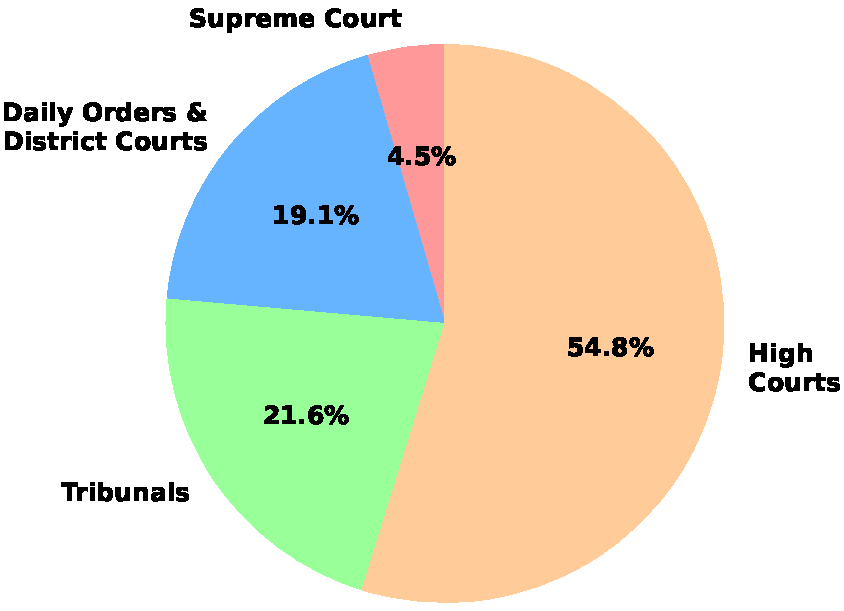
\includegraphics[width=\columnwidth]{figures/Distribution_of_Cases_in_Courts.pdf}
    \caption{Distribution of cases in different courts.}
    \label{fig:court-distribution}
\end{figure}
%%%%%%%%%%%%%%%%%%%%%%%%%%%%%%%%%%%%
\section{Preprocessing}
The preprocessing of the \texttt{\named} dataset involved several critical steps to ensure the data's quality and relevance. Given the unstructured nature of the documents, which varied in format and size, we faced challenges such as spelling errors and inconsistencies. To mitigate these, we used regular expressions to remove noisy text and meta-information, including case numbers, titles, judge names, petitioners, respondents, and dates. We identified key sections using specific terms like `ORDER,' `JUDGMENT,' and `JUDGEMENT' to isolate the essential content and filter out irrelevant details.

We further refined the dataset by removing cases without clear outcomes or insufficient information. To maintain consistency and manageability, we excluded extremely short cases (less than 50 words) and excessively long ones (more than 32,000 words). Additionally, tokens with characters repeated more than twice consecutively were removed to clean up text errors. This meticulous refinement process reduced the number of cases to 11,25,604, retaining only the most relevant cases, as detailed in Table \ref{tab:before-and-after}, which compares the number of cases before and after preprocessing, categorized by court type.

\subsection{Label Making}
After filtering, the documents were labeled using keywords indicative of positive outcomes like ``approved," ``allowed," and ``granted," or negative outcomes such as ``rejected," ``disapproved," and ``dismissed." This labeling process helped classify the cases into likely acceptance or rejection categories. We categorized the cases into two groups: single-labeled cases, where all appeals had the same outcome or only a single appeal was filed, marked as 0 (rejection) or 1 (acceptance), and multi-labeled judgments, where at least one appeal was accepted, indicating partial acceptance, marked as 2.

To ensure accurate labeling, we focused on the last 750 words of each document, typically where decisions are summarized. Special attention was given to a context window around key terms like ``appeal," ``petition," or ``case" to accurately determine the judgment nature. For example, phrases like ``Appeals Allowed" or ``The appeal is granted" indicated a positive outcome, while ``The appeal has no proper evidence and hence we reject it" indicated rejection. We also looked for indicators like ``partly" to identify multi-labeled judgments for cases with partial approvals. In instances where the judgment was phrased negatively (e.g., ``No appeal is allowed"), we used a label-flipping strategy if negation words like ``no" or ``not" were found close to key terms, ensuring the labels accurately reflected the judgment's intent.

This meticulous approach to labeling, focusing on the judgment's context and nuanced expression, enhances the reliability of our dataset and prepares it for effective training of judgment prediction models.

%%%%%%%%%%%%%%%%%%%%%%%%%%%%%%%%%%%%
\begin{figure*}[t] % [h] specifies the placement of the figure NyayaAnumana_Flow.drawio_new.pdf ->NyayaAnumana_Flow.drawio (2).drawio.pdf->NyayaAnumana_Flow.drawio (2).drawio (3).pdf
    \centering % Centers the figure
    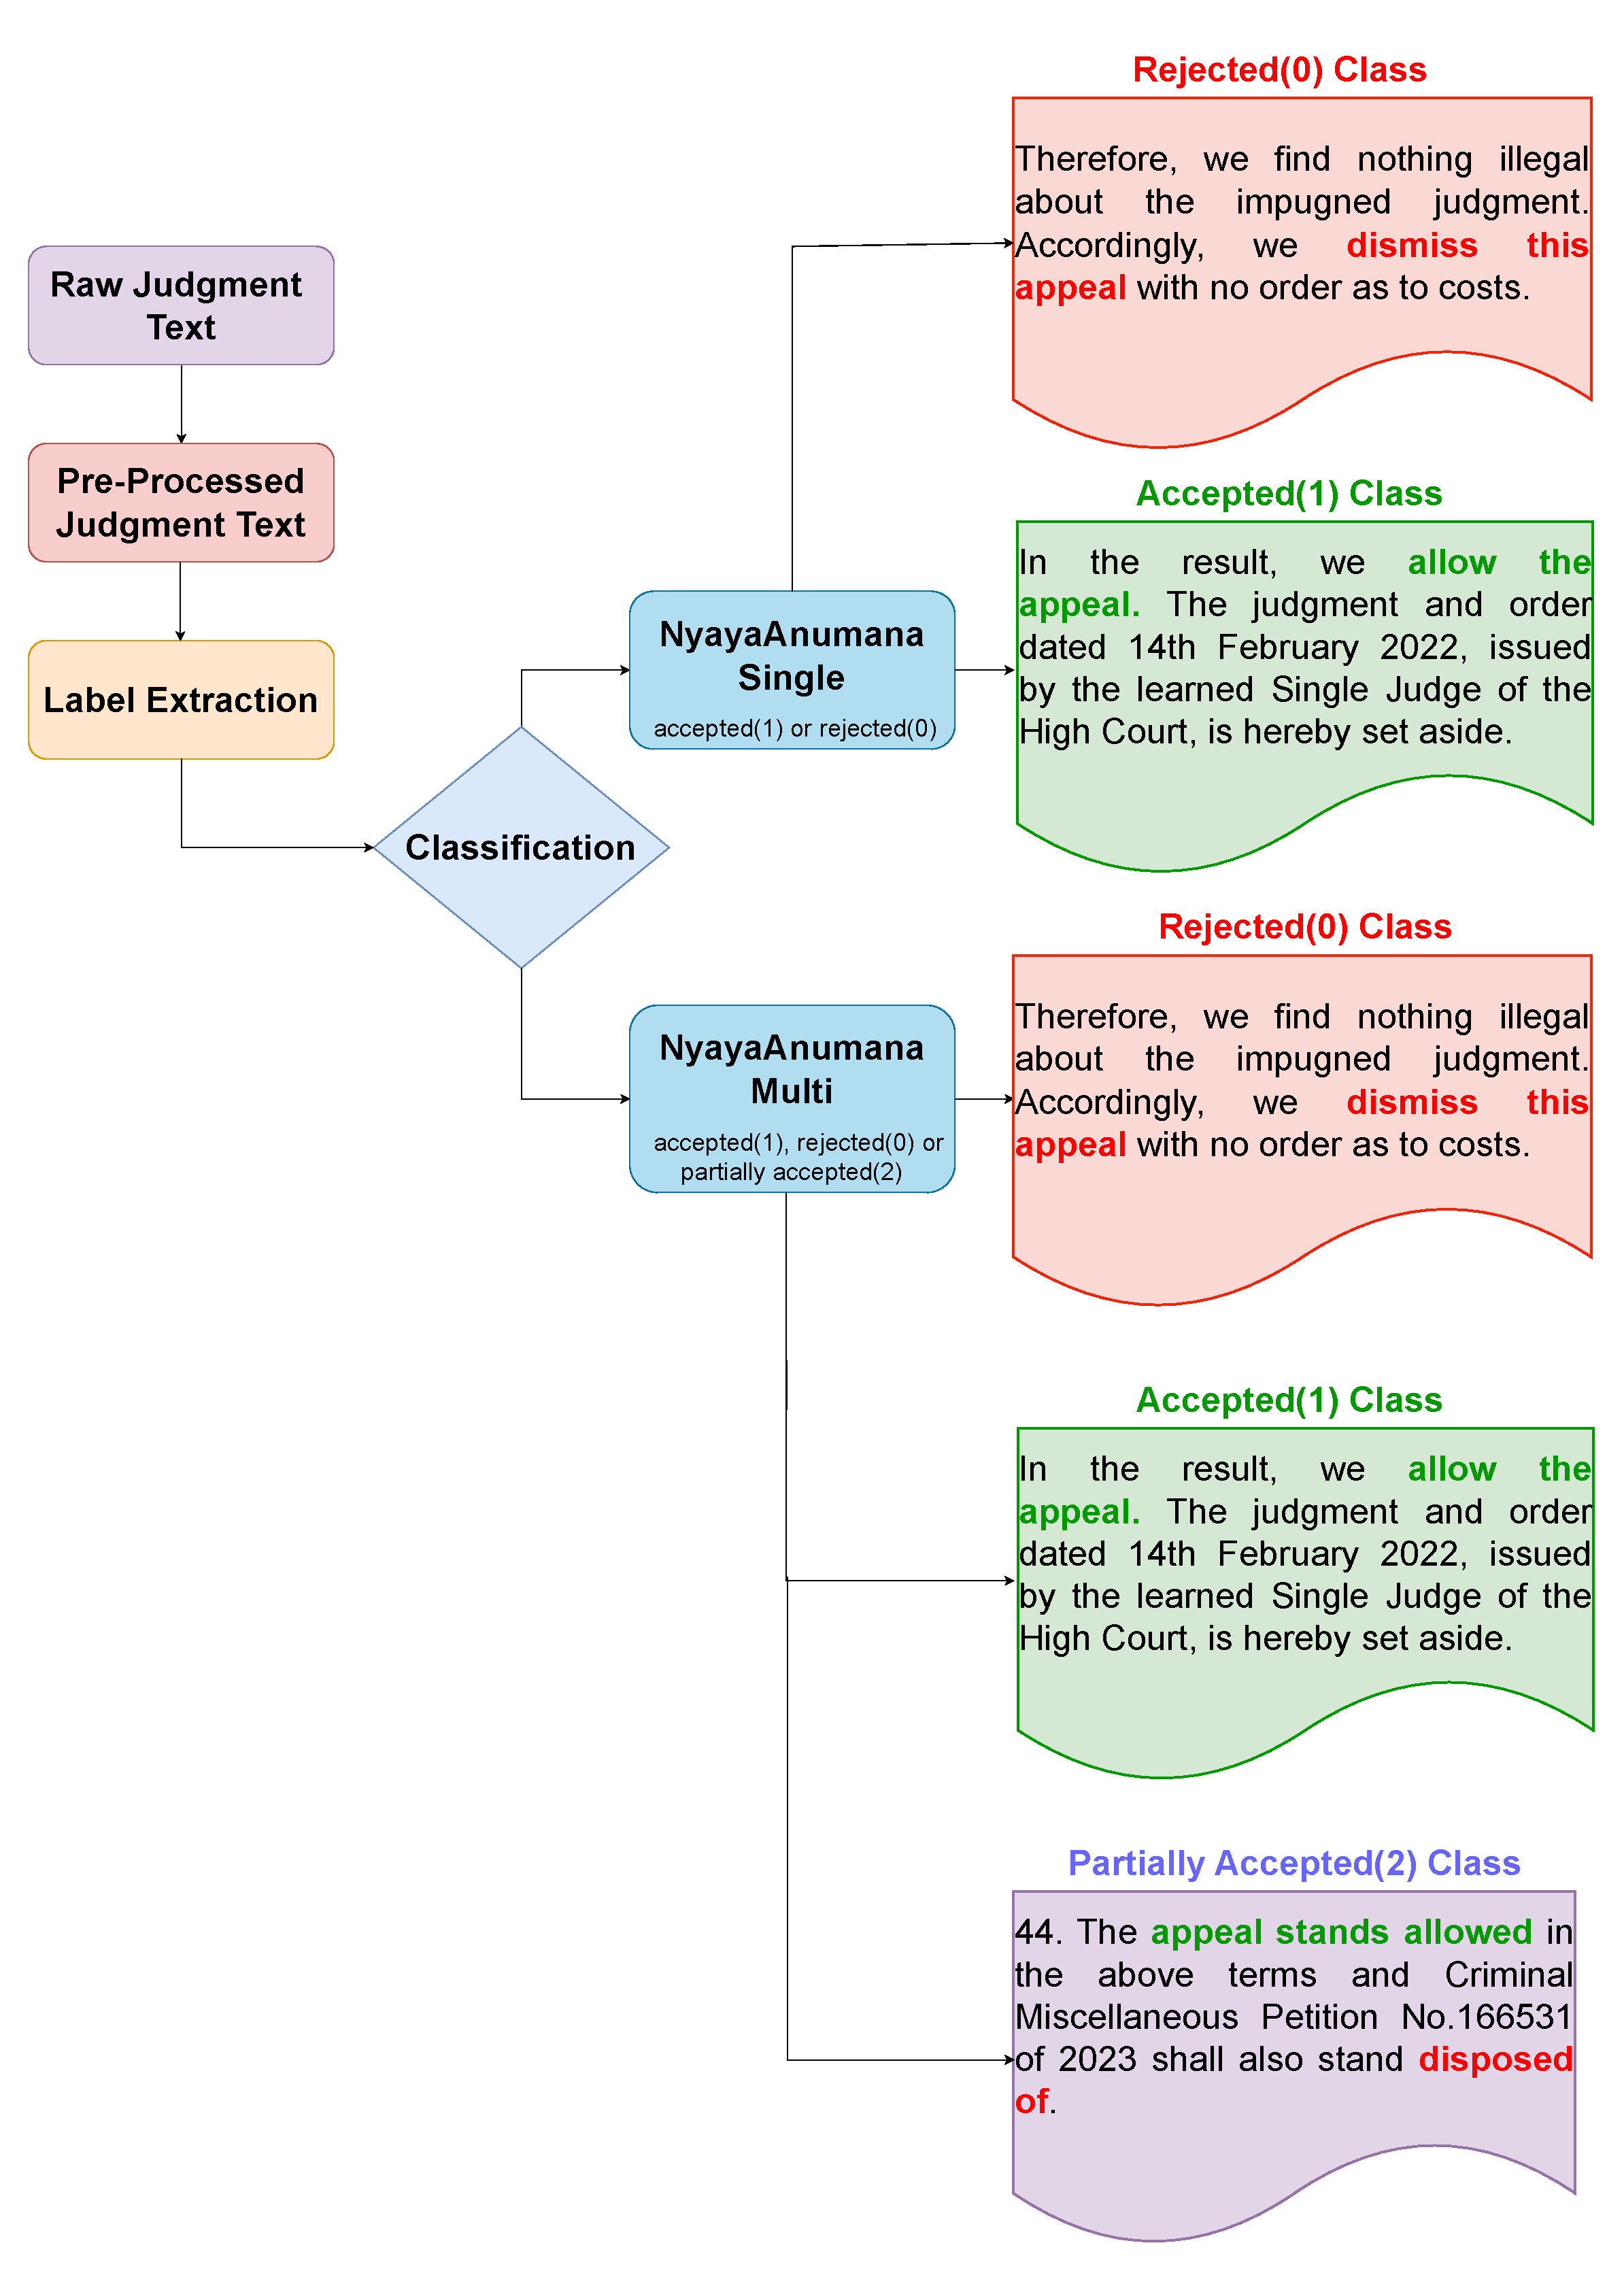
\includegraphics[width=\linewidth]{figures/NyayaAnumana_Flow.pdf} % Adjust width as needed
  
    \caption{Illustration of the LJP Task Framework.}
    \label{fig:task-framework} % For referencing the figure
\end{figure*}
%%%%%%%%%%%%%%%%%%%%%%%%%%%%%%%%%%%%

%%%%%%%%%%%%%%%%%%%%%%%%%%%%%%%%%%%%%%%%%%%%%%%
\begin{table}[ht]
\centering
\resizebox{\columnwidth}{!}{%
\begin{tabular}{lrrr}
\hline
\textbf{Court-wise} &
  \textbf{Raw files} &
  \textbf{\begin{tabular}[c]{@{}c@{}}FIles After \\ Preprocessing\end{tabular}} &
  \textbf{\begin{tabular}[c]{@{}c@{}}FIles After \\ Lebeling\end{tabular}} \\ \hline
\textbf{Supreme Court}  & 55,928   & 54,831   & 40,562  \\
\textbf{High Court}     & 13,24,373 & 9,77,849  & 4,82,295 \\
\textbf{Tribunal Court} & 4,77,397  & 3,18,681  & 1,86,671 \\
\textbf{\begin{tabular}[c]{@{}l@{}}Daily Orders and\\ District Courts\end{tabular}}    & 4,24,439  & 3,12,480  & 92,771 \\ 
\hline
\textbf{Total}          & 22,82,137 & 16,63,841 & 8,02,299
\\ \hline
\end{tabular}%
}
\caption{Number of cases before and after preprocessing, by court type.}
\label{tab:before-and-after}
\end{table}
%%%%%%%%%%%%%%%%%%%%%%%%%%%%%%%%%%%%%%%%%%%%%%%

%%%%%%%%%%%%%%%%%%%%%%%%%
% Legal Expert Ratings
%%%%%%%%%%%%%%%%%%%%%%%%%%%%%%%%%%

\begin{table}[t]
\centering
\resizebox{0.8\columnwidth}{!}{%
\begin{tabular}{lccccc}
%\hline\
\toprule
 &
  \multicolumn{5}{c}{\textbf{Rating Score}} \\ \midrule%\hline
 
 &
  \multicolumn{1}{c}{\textbf{1}} &
  \multicolumn{1}{c}{\textbf{2}} &
  \multicolumn{1}{c}{\textbf{3}} &
  \multicolumn{1}{c}{\textbf{4}} &
  \textbf{5} \\ \cline{2-6} 
 
\multirow{-2}{*}{\textbf{Generative Models}} &
  \multicolumn{5}{c}{\textbf{PredEx}} \\ \midrule%\hline
LLaMa-2-7B &
  \multicolumn{1}{c}{{ 2}} &
  \multicolumn{1}{c}{{ 11}} &
  \multicolumn{1}{c}{{ 22}} &
  \multicolumn{1}{c}{{ 12}} &
  { 3} \\ %\hline
\begin{tabular}[c]{@{}l@{}}LLaMa-2 SFT\end{tabular} &
  \multicolumn{1}{c}{{ 5}} &
  \multicolumn{1}{c}{13} &
  \multicolumn{1}{c}{18} &
  \multicolumn{1}{c}{13} &
  1 \\ %\hline

\begin{tabular}[c]{@{}l@{}}LLaMa-2 CPT\end{tabular} &
  \multicolumn{1}{c}{{ 2}} &
  \multicolumn{1}{c}{2} &
  \multicolumn{1}{c}{27} &
  \multicolumn{1}{c}{19} &
  0 \\ %\hline

\begin{tabular}[c]{@{}l@{}}\textbf{\namel} \\\textbf{CPT+SFT}\end{tabular} &
  \multicolumn{1}{c}{{ 0}} &
  \multicolumn{1}{c}{0} &
  \multicolumn{1}{c}{23} &
  \multicolumn{1}{c}{27} &
  0 \\ \midrule%\hline
 &
  \multicolumn{5}{c}{\textbf{ILDC\_expert}} \\ \midrule%\hline
LLaMa-2-7B &
  \multicolumn{1}{c}{0} &
  \multicolumn{1}{c}{9} &
  \multicolumn{1}{c}{22} &
  \multicolumn{1}{c}{21} &
  2 \\ %\hline
\begin{tabular}[c]{@{}l@{}}LLaMa-2 SFT\end{tabular} &
  \multicolumn{1}{c}{2} &
  \multicolumn{1}{c}{3} &
  \multicolumn{1}{c}{16} &
  \multicolumn{1}{c}{24} &
  9 \\ %\hline

  \begin{tabular}[c]{@{}l@{}}LLaMa-2 CPT\end{tabular} &
  \multicolumn{1}{c}{{1}} &
  \multicolumn{1}{c}{3} &
  \multicolumn{1}{c}{25} &
  \multicolumn{1}{c}{23} &
  2 \\ %\hline

\begin{tabular}[c]{@{}l@{}}\textbf{\namel} \\\textbf{CPT+SFT}\end{tabular} &
  \multicolumn{1}{c}{{ 0}} &
  \multicolumn{1}{c}{0} &
  \multicolumn{1}{c}{22} &
  \multicolumn{1}{c}{28} &
  4 \\ \bottomrule%\hline
\end{tabular}%
}
\caption{Distribution of Expert Rating Scores for Generative Models on PredEx and ILDC\_expert Data.}
\label{expert-scores}
\end{table}
%%%%%%%%%%%%%%%%%%%%%%%%%